\hypertarget{_t96mod_8f}{
\section{/home/mgh/LanlGeoMag/libLanlGeoMag/T96mod.f File Reference}
\label{_t96mod_8f}\index{/home/mgh/LanlGeoMag/libLanlGeoMag/T96mod.f@{/home/mgh/LanlGeoMag/libLanlGeoMag/T96mod.f}}
}
\subsection*{Functions}
\begin{CompactItemize}
\item 
subroutine \hyperlink{_t96mod_8f_d1b3c77658e29c0a582e4458288a48a7}{T96MOD} (IOPT, PARMOD, PS, X, Y, Z, BX, BY, BZ)
\item 
subroutine \hyperlink{_t96mod_8f_7194bba01ce7c686c27501da1f6e23a8}{T96\_\-01} (IOPT, PARMOD, PS, X, Y, Z, BX, BY, BZ)
\item 
subroutine \hyperlink{_t96mod_8f_22b5155440601bb1258e41b0407b707f}{DIPSHLD} (PS, X, Y, Z, BX, BY, BZ)
\item 
subroutine \hyperlink{_t96mod_8f_a1021262eae38287e65bc7ff696f67a2}{CYLHARM} (A, X, Y, Z, BX, BY, BZ)
\item 
subroutine \hyperlink{_t96mod_8f_79feb4cb40c2a7d62058e92afda49cf6}{CYLHAR1} (A, X, Y, Z, BX, BY, BZ)
\item 
DOUBLE PRECISION \hyperlink{_t96mod_8f_273ee53e86263995858fc8c0a702433a}{BES} (X, K)
\item 
DOUBLE PRECISION \hyperlink{_t96mod_8f_bc4ab00dda905b70971f5b3dae102841}{BES0} (X)
\item 
DOUBLE PRECISION \hyperlink{_t96mod_8f_5dd1f9e8738676c1ded360e252f7ef48}{BES1} (X)
\item 
subroutine \hyperlink{_t96mod_8f_2e097fa1f961156bc2ca8b94983b9e4f}{INTERCON} (X, Y, Z, BX, BY, BZ)
\item 
subroutine \hyperlink{_t96mod_8f_a2c7e086277c827ff05f4a9c6eb99b2b}{TAILRC96} (DMODIF, SPS, X, Y, Z, BXRC, BYRC, BZRC, BXT2, BYT2,$\ast$BZT2, BXT3, BYT3, BZT3, BXT2ADD, BYT2ADD, BZT2ADD)
\item 
subroutine \hyperlink{_t96mod_8f_87fae8404610c1e792fff8db728b60a3}{RINGCURR96} (X, Y, Z, BX, BY, BZ)
\item 
subroutine \hyperlink{_t96mod_8f_b0a52ce0e8651f818014bb9cd0040927}{T96MOD\_\-TAILDISK} (X, Y, Z, BX, BY, BZ)
\item 
subroutine \hyperlink{_t96mod_8f_cbb331c88d418399755655497d909b64}{T96MOD\_\-TAILDISKADD} (DMODIF, X, Y, Z, BX, BY, BZ)
\item 
subroutine \hyperlink{_t96mod_8f_f7a0147645dfe77e8197e10963ed3770}{TAIL87} (X, Z, BX, BZ)
\item 
subroutine \hyperlink{_t96mod_8f_0918ae2ac8568570f93f2d5c0d88f9dc}{T96MOD\_\-SHLCAR3X3} (A, X, Y, Z, SPS, HX, HY, HZ)
\item 
subroutine \hyperlink{_t96mod_8f_1d35065857c1597a4d45699d6e30faa9}{BIRK1TOT\_\-02} (PS, X, Y, Z, BX, BY, BZ)
\item 
subroutine \hyperlink{_t96mod_8f_7634ccf219c90ebc36de1b55b961ed88}{DIPLOOP1} (XI, D)
\item 
subroutine \hyperlink{_t96mod_8f_7ad3cc17a6906d0de0ea87905c8adfa0}{CIRCLE} (X, Y, Z, RL, BX, BY, BZ)
\item 
subroutine \hyperlink{_t96mod_8f_339de23a7fc16677d5c934050601456b}{CROSSLP} (X, Y, Z, BX, BY, BZ, XC, RL, AL)
\item 
subroutine \hyperlink{_t96mod_8f_76f3ffff48346c7a53f738f013945222}{DIPXYZ} (X, Y, Z, BXX, BYX, BZX, BXY, BYY, BZY, BXZ, BYZ, BZZ)
\item 
subroutine \hyperlink{_t96mod_8f_2432dab29def6a7f82b4e61542784ca2}{CONDIP1} (XI, D)
\item 
subroutine \hyperlink{_t96mod_8f_e7df392ea162336df5811079016b08ac}{BIRK1SHLD} (PS, X, Y, Z, BX, BY, BZ)
\item 
subroutine \hyperlink{_t96mod_8f_72d9123c4c7f8cc57e525a533b45d5fe}{BIRK2TOT\_\-02} (PS, X, Y, Z, BX, BY, BZ)
\item 
subroutine \hyperlink{_t96mod_8f_09ee39e02874a680b5fe915e9ccbc8f6}{BIRK2SHL} (X, Y, Z, PS, HX, HY, HZ)
\item 
subroutine \hyperlink{_t96mod_8f_75644447b8b698b1ea33e1bc67aba7af}{R2\_\-BIRK} (X, Y, Z, PS, BX, BY, BZ)
\item 
subroutine \hyperlink{_t96mod_8f_717e6c5b669e682bef3f33b1a4a73796}{R2INNER} (X, Y, Z, BX, BY, BZ)
\item 
subroutine \hyperlink{_t96mod_8f_1a6fae1af90cf34b2b4e95d5ecde87a9}{BCONIC} (X, Y, Z, CBX, CBY, CBZ, NMAX)
\item 
subroutine \hyperlink{_t96mod_8f_26863a8d653e16bfa831cf1cd3d57367}{DIPDISTR} (X, Y, Z, BX, BY, BZ, MODE)
\item 
subroutine \hyperlink{_t96mod_8f_4b792e262830f77251236192fe6ade49}{R2OUTER} (X, Y, Z, BX, BY, BZ)
\item 
subroutine \hyperlink{_t96mod_8f_8bb46e1322b561a6e5aa91de2b85a0e2}{LOOPS4} (X, Y, Z, BX, BY, BZ, XC, YC, ZC, R, THETA, PHI)
\item 
subroutine \hyperlink{_t96mod_8f_d2c23a8a964ae249deaa1665da76803f}{R2SHEET} (X, Y, Z, BX, BY, BZ)
\item 
DOUBLE PRECISION \hyperlink{_t96mod_8f_34df9615369af608c58c50830a71bc2c}{XKSI} (X, Y, Z)
\item 
function \hyperlink{_t96mod_8f_de7e8858bac24c4e9ef3bbee7949e235}{FEXP} (S, A)
\item 
function \hyperlink{_t96mod_8f_4652a5d7098ea16cd1f49a0597effa56}{FEXP1} (S, A)
\item 
DOUBLE PRECISION \hyperlink{_t96mod_8f_2b6a113bedd0458c72d9e0723c3bb7d4}{TKSI} (XKSI, XKS0, DXKSI)
\item 
subroutine \hyperlink{_t96mod_8f_39c75fa7da285932d582aadcf8a2442d}{T96MOD\_\-DIPOLE} (PS, X, Y, Z, BX, BY, BZ)
\end{CompactItemize}


\subsection{Function Documentation}
\hypertarget{_t96mod_8f_d1b3c77658e29c0a582e4458288a48a7}{
\index{T96mod.f@{T96mod.f}!T96MOD@{T96MOD}}
\index{T96MOD@{T96MOD}!T96mod.f@{T96mod.f}}
\subsubsection[{T96MOD}]{\setlength{\rightskip}{0pt plus 5cm}subroutine T96MOD (IOPT, \/  REAL$\ast$8,dimension(10) {\em PARMOD}, \/  REAL$\ast$8 {\em PS}, \/  REAL$\ast$8 {\em X}, \/  REAL$\ast$8 {\em Y}, \/  REAL$\ast$8 {\em Z}, \/  REAL$\ast$8 {\em BX}, \/  REAL$\ast$8 {\em BY}, \/  REAL$\ast$8 {\em BZ})}}
\label{_t96mod_8f_d1b3c77658e29c0a582e4458288a48a7}




Definition at line 8 of file T96mod.f.

Here is the call graph for this function:\nopagebreak
\begin{figure}[H]
\begin{center}
\leavevmode
\includegraphics[width=343pt]{_t96mod_8f_d1b3c77658e29c0a582e4458288a48a7_cgraph}
\end{center}
\end{figure}


Here is the caller graph for this function:\nopagebreak
\begin{figure}[H]
\begin{center}
\leavevmode
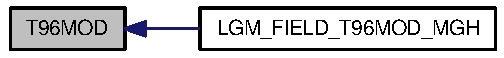
\includegraphics[width=139pt]{_t96mod_8f_d1b3c77658e29c0a582e4458288a48a7_icgraph}
\end{center}
\end{figure}
\hypertarget{_t96mod_8f_7194bba01ce7c686c27501da1f6e23a8}{
\index{T96mod.f@{T96mod.f}!T96\_\-01@{T96\_\-01}}
\index{T96\_\-01@{T96\_\-01}!T96mod.f@{T96mod.f}}
\subsubsection[{T96\_\-01}]{\setlength{\rightskip}{0pt plus 5cm}subroutine T96\_\-01 (IOPT, \/  REAL$\ast$8,dimension(10) {\em PARMOD}, \/  REAL$\ast$8 {\em PS}, \/  REAL$\ast$8 {\em X}, \/  REAL$\ast$8 {\em Y}, \/  REAL$\ast$8 {\em Z}, \/  REAL$\ast$8 {\em BX}, \/  REAL$\ast$8 {\em BY}, \/  REAL$\ast$8 {\em BZ})}}
\label{_t96mod_8f_7194bba01ce7c686c27501da1f6e23a8}




Definition at line 197 of file T96mod.f.

Here is the call graph for this function:\nopagebreak
\begin{figure}[H]
\begin{center}
\leavevmode
\includegraphics[width=339pt]{_t96mod_8f_7194bba01ce7c686c27501da1f6e23a8_cgraph}
\end{center}
\end{figure}
\hypertarget{_t96mod_8f_22b5155440601bb1258e41b0407b707f}{
\index{T96mod.f@{T96mod.f}!DIPSHLD@{DIPSHLD}}
\index{DIPSHLD@{DIPSHLD}!T96mod.f@{T96mod.f}}
\subsubsection[{DIPSHLD}]{\setlength{\rightskip}{0pt plus 5cm}subroutine DIPSHLD (PS, \/  X, \/  Y, \/  Z, \/  BX, \/  BY, \/  BZ)}}
\label{_t96mod_8f_22b5155440601bb1258e41b0407b707f}




Definition at line 375 of file T96mod.f.

Here is the call graph for this function:\nopagebreak
\begin{figure}[H]
\begin{center}
\leavevmode
\includegraphics[width=178pt]{_t96mod_8f_22b5155440601bb1258e41b0407b707f_cgraph}
\end{center}
\end{figure}


Here is the caller graph for this function:\nopagebreak
\begin{figure}[H]
\begin{center}
\leavevmode
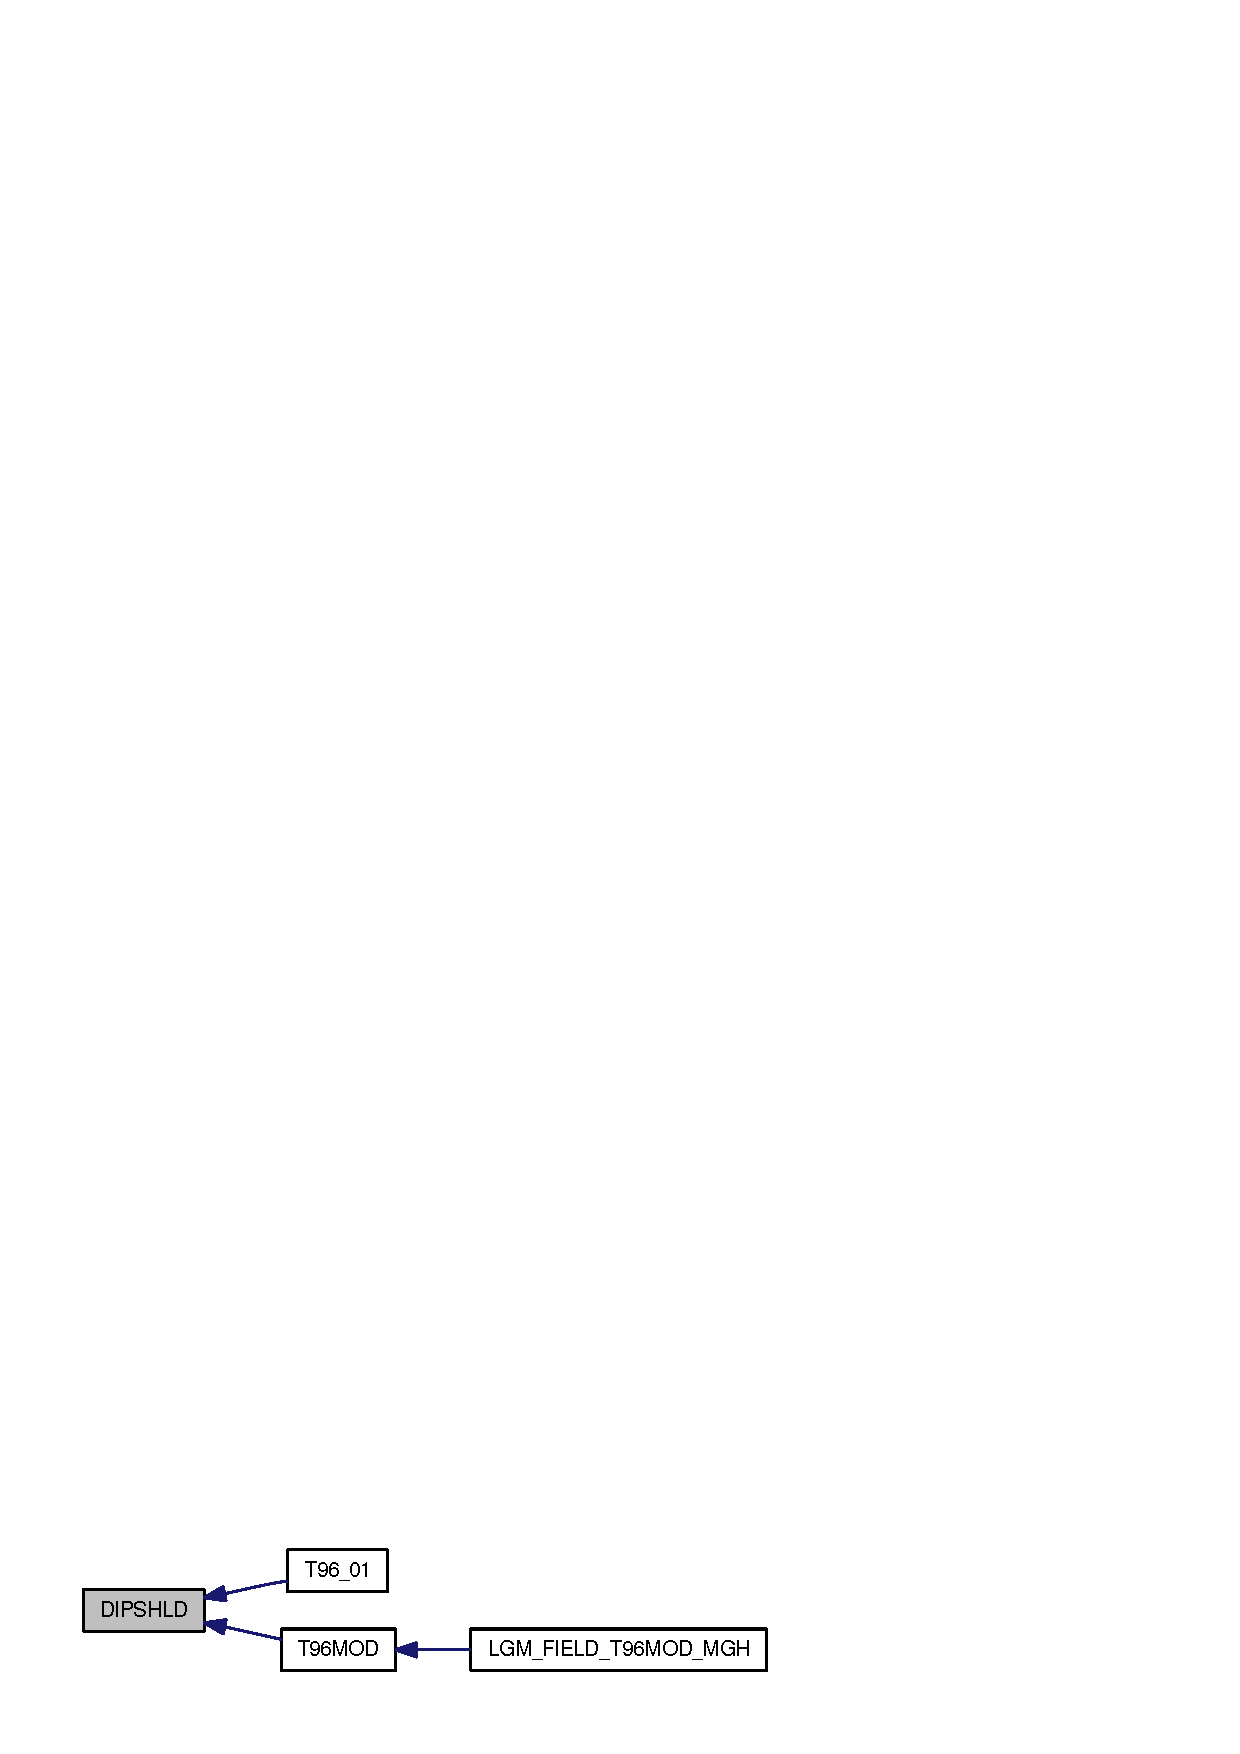
\includegraphics[width=186pt]{_t96mod_8f_22b5155440601bb1258e41b0407b707f_icgraph}
\end{center}
\end{figure}
\hypertarget{_t96mod_8f_a1021262eae38287e65bc7ff696f67a2}{
\index{T96mod.f@{T96mod.f}!CYLHARM@{CYLHARM}}
\index{CYLHARM@{CYLHARM}!T96mod.f@{T96mod.f}}
\subsubsection[{CYLHARM}]{\setlength{\rightskip}{0pt plus 5cm}subroutine CYLHARM (A, \/  X, \/  Y, \/  Z, \/  BX, \/  BY, \/  BZ)}}
\label{_t96mod_8f_a1021262eae38287e65bc7ff696f67a2}




Definition at line 402 of file T96mod.f.

Here is the call graph for this function:\nopagebreak
\begin{figure}[H]
\begin{center}
\leavevmode
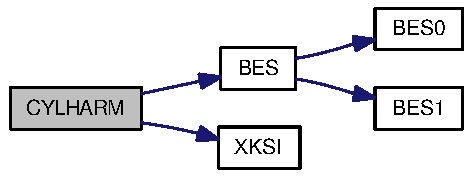
\includegraphics[width=131pt]{_t96mod_8f_a1021262eae38287e65bc7ff696f67a2_cgraph}
\end{center}
\end{figure}


Here is the caller graph for this function:\nopagebreak
\begin{figure}[H]
\begin{center}
\leavevmode
\includegraphics[width=236pt]{_t96mod_8f_a1021262eae38287e65bc7ff696f67a2_icgraph}
\end{center}
\end{figure}
\hypertarget{_t96mod_8f_79feb4cb40c2a7d62058e92afda49cf6}{
\index{T96mod.f@{T96mod.f}!CYLHAR1@{CYLHAR1}}
\index{CYLHAR1@{CYLHAR1}!T96mod.f@{T96mod.f}}
\subsubsection[{CYLHAR1}]{\setlength{\rightskip}{0pt plus 5cm}subroutine CYLHAR1 (A, \/  X, \/  Y, \/  Z, \/  BX, \/  BY, \/  BZ)}}
\label{_t96mod_8f_79feb4cb40c2a7d62058e92afda49cf6}




Definition at line 475 of file T96mod.f.

Here is the call graph for this function:\nopagebreak
\begin{figure}[H]
\begin{center}
\leavevmode
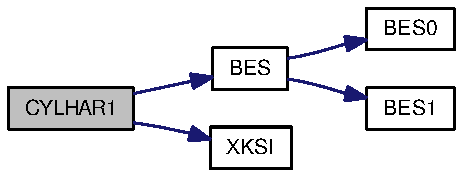
\includegraphics[width=129pt]{_t96mod_8f_79feb4cb40c2a7d62058e92afda49cf6_cgraph}
\end{center}
\end{figure}


Here is the caller graph for this function:\nopagebreak
\begin{figure}[H]
\begin{center}
\leavevmode
\includegraphics[width=234pt]{_t96mod_8f_79feb4cb40c2a7d62058e92afda49cf6_icgraph}
\end{center}
\end{figure}
\hypertarget{_t96mod_8f_273ee53e86263995858fc8c0a702433a}{
\index{T96mod.f@{T96mod.f}!BES@{BES}}
\index{BES@{BES}!T96mod.f@{T96mod.f}}
\subsubsection[{BES}]{\setlength{\rightskip}{0pt plus 5cm}DOUBLE PRECISION BES (X, \/  K)}}
\label{_t96mod_8f_273ee53e86263995858fc8c0a702433a}




Definition at line 545 of file T96mod.f.

Here is the call graph for this function:\nopagebreak
\begin{figure}[H]
\begin{center}
\leavevmode
\includegraphics[width=79pt]{_t96mod_8f_273ee53e86263995858fc8c0a702433a_cgraph}
\end{center}
\end{figure}


Here is the caller graph for this function:\nopagebreak
\begin{figure}[H]
\begin{center}
\leavevmode
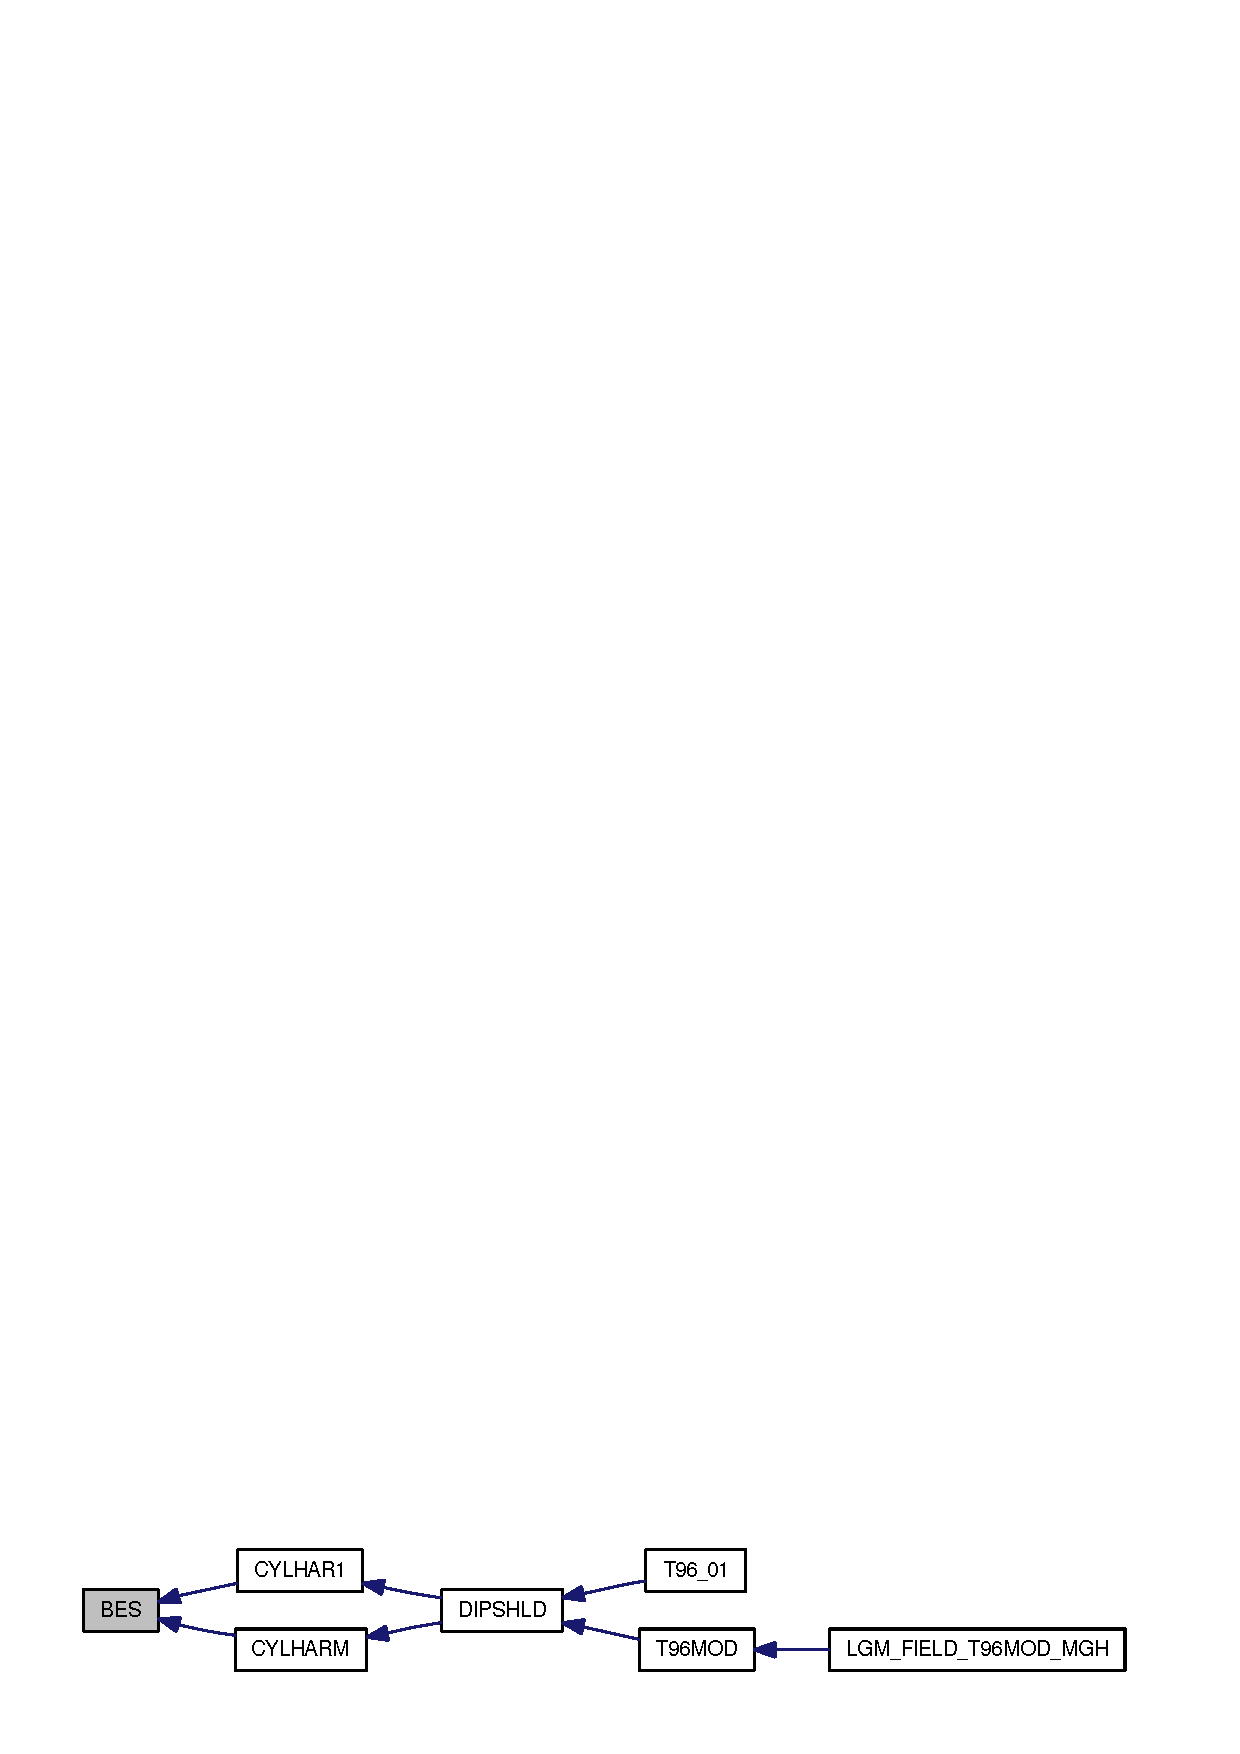
\includegraphics[width=272pt]{_t96mod_8f_273ee53e86263995858fc8c0a702433a_icgraph}
\end{center}
\end{figure}
\hypertarget{_t96mod_8f_bc4ab00dda905b70971f5b3dae102841}{
\index{T96mod.f@{T96mod.f}!BES0@{BES0}}
\index{BES0@{BES0}!T96mod.f@{T96mod.f}}
\subsubsection[{BES0}]{\setlength{\rightskip}{0pt plus 5cm}DOUBLE PRECISION BES0 (X)}}
\label{_t96mod_8f_bc4ab00dda905b70971f5b3dae102841}




Definition at line 609 of file T96mod.f.

Here is the caller graph for this function:\nopagebreak
\begin{figure}[H]
\begin{center}
\leavevmode
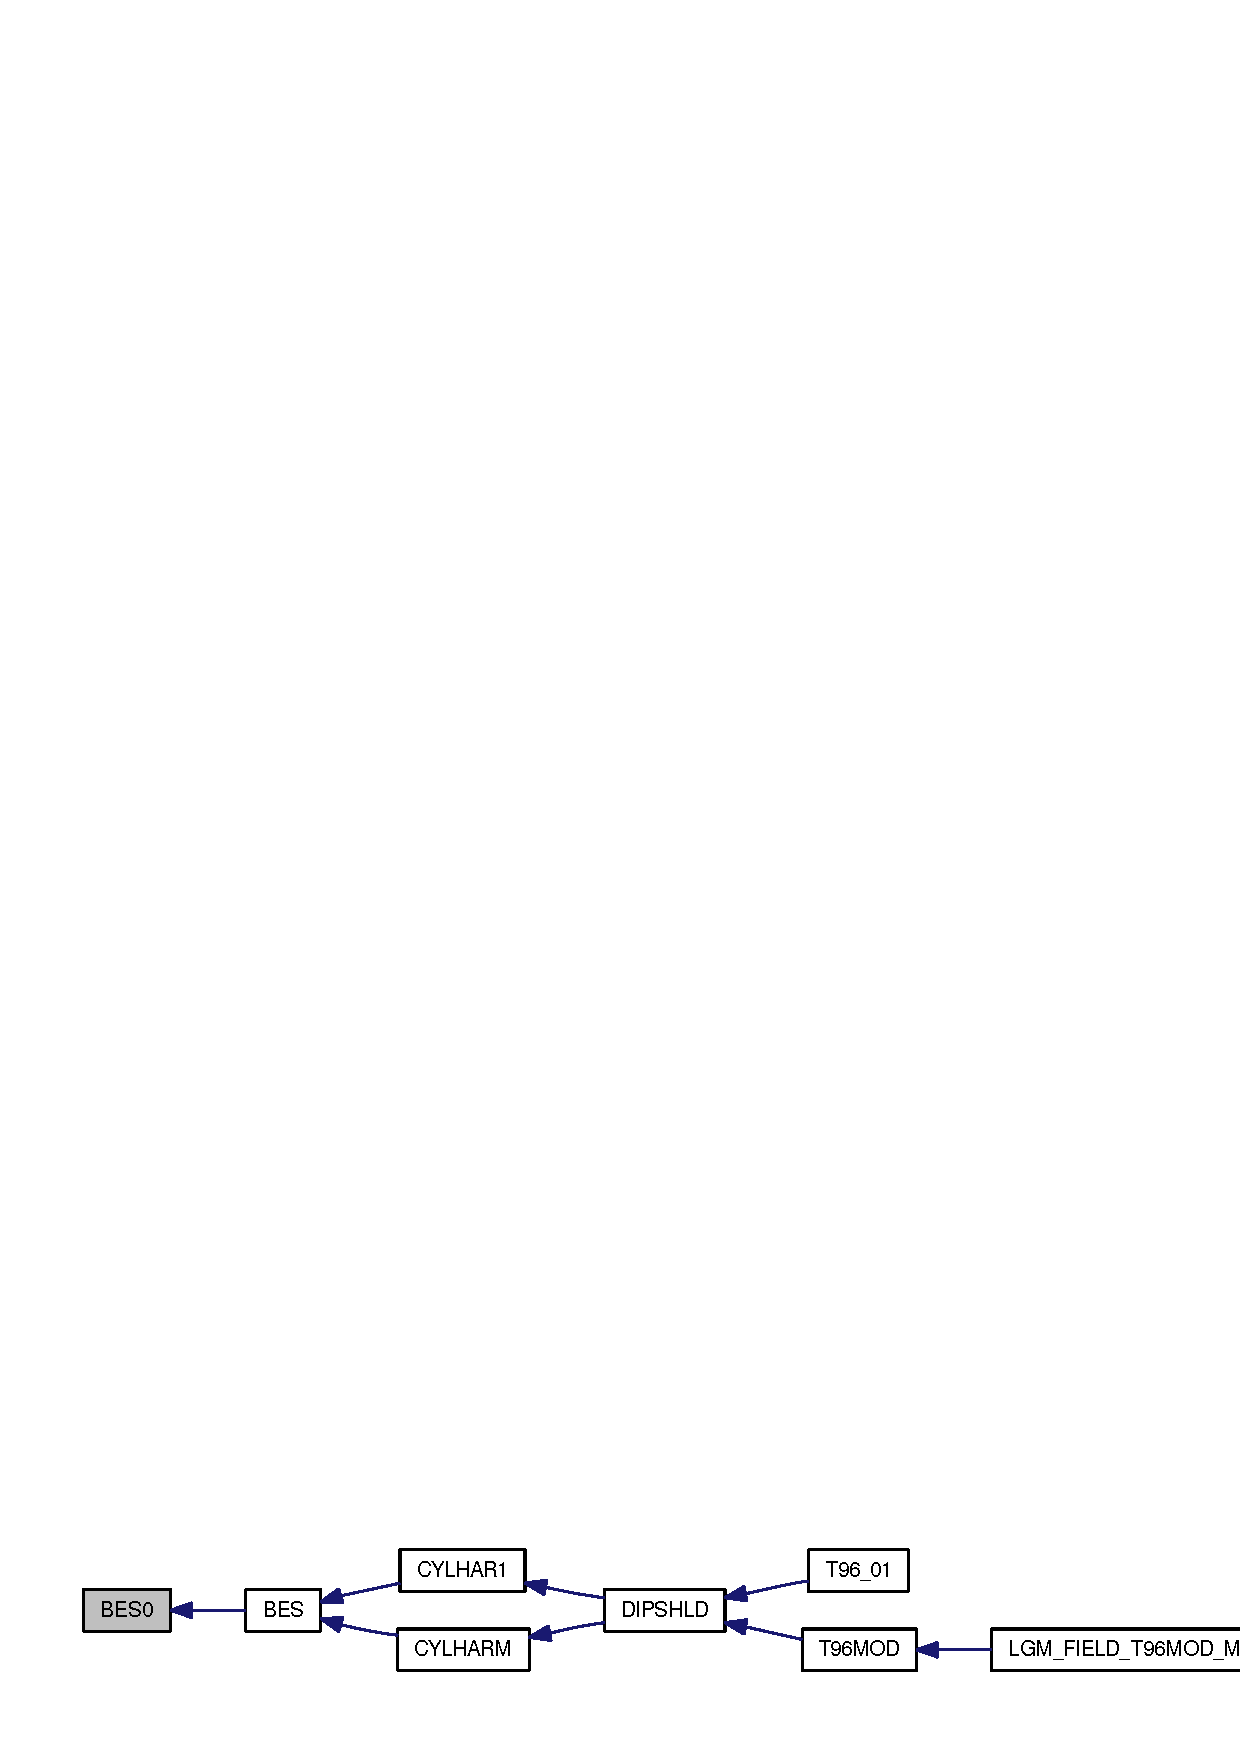
\includegraphics[width=311pt]{_t96mod_8f_bc4ab00dda905b70971f5b3dae102841_icgraph}
\end{center}
\end{figure}
\hypertarget{_t96mod_8f_5dd1f9e8738676c1ded360e252f7ef48}{
\index{T96mod.f@{T96mod.f}!BES1@{BES1}}
\index{BES1@{BES1}!T96mod.f@{T96mod.f}}
\subsubsection[{BES1}]{\setlength{\rightskip}{0pt plus 5cm}DOUBLE PRECISION BES1 (X)}}
\label{_t96mod_8f_5dd1f9e8738676c1ded360e252f7ef48}




Definition at line 633 of file T96mod.f.

Here is the caller graph for this function:\nopagebreak
\begin{figure}[H]
\begin{center}
\leavevmode
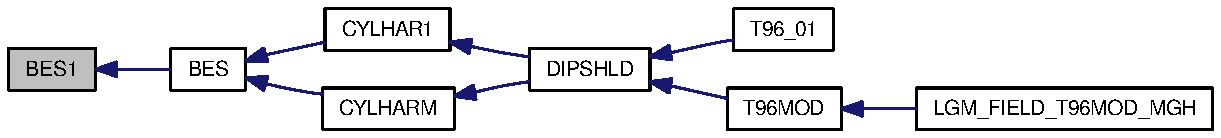
\includegraphics[width=311pt]{_t96mod_8f_5dd1f9e8738676c1ded360e252f7ef48_icgraph}
\end{center}
\end{figure}
\hypertarget{_t96mod_8f_2e097fa1f961156bc2ca8b94983b9e4f}{
\index{T96mod.f@{T96mod.f}!INTERCON@{INTERCON}}
\index{INTERCON@{INTERCON}!T96mod.f@{T96mod.f}}
\subsubsection[{INTERCON}]{\setlength{\rightskip}{0pt plus 5cm}subroutine INTERCON (X, \/  Y, \/  Z, \/  BX, \/  BY, \/  BZ)}}
\label{_t96mod_8f_2e097fa1f961156bc2ca8b94983b9e4f}




Definition at line 657 of file T96mod.f.

Here is the caller graph for this function:\nopagebreak
\begin{figure}[H]
\begin{center}
\leavevmode
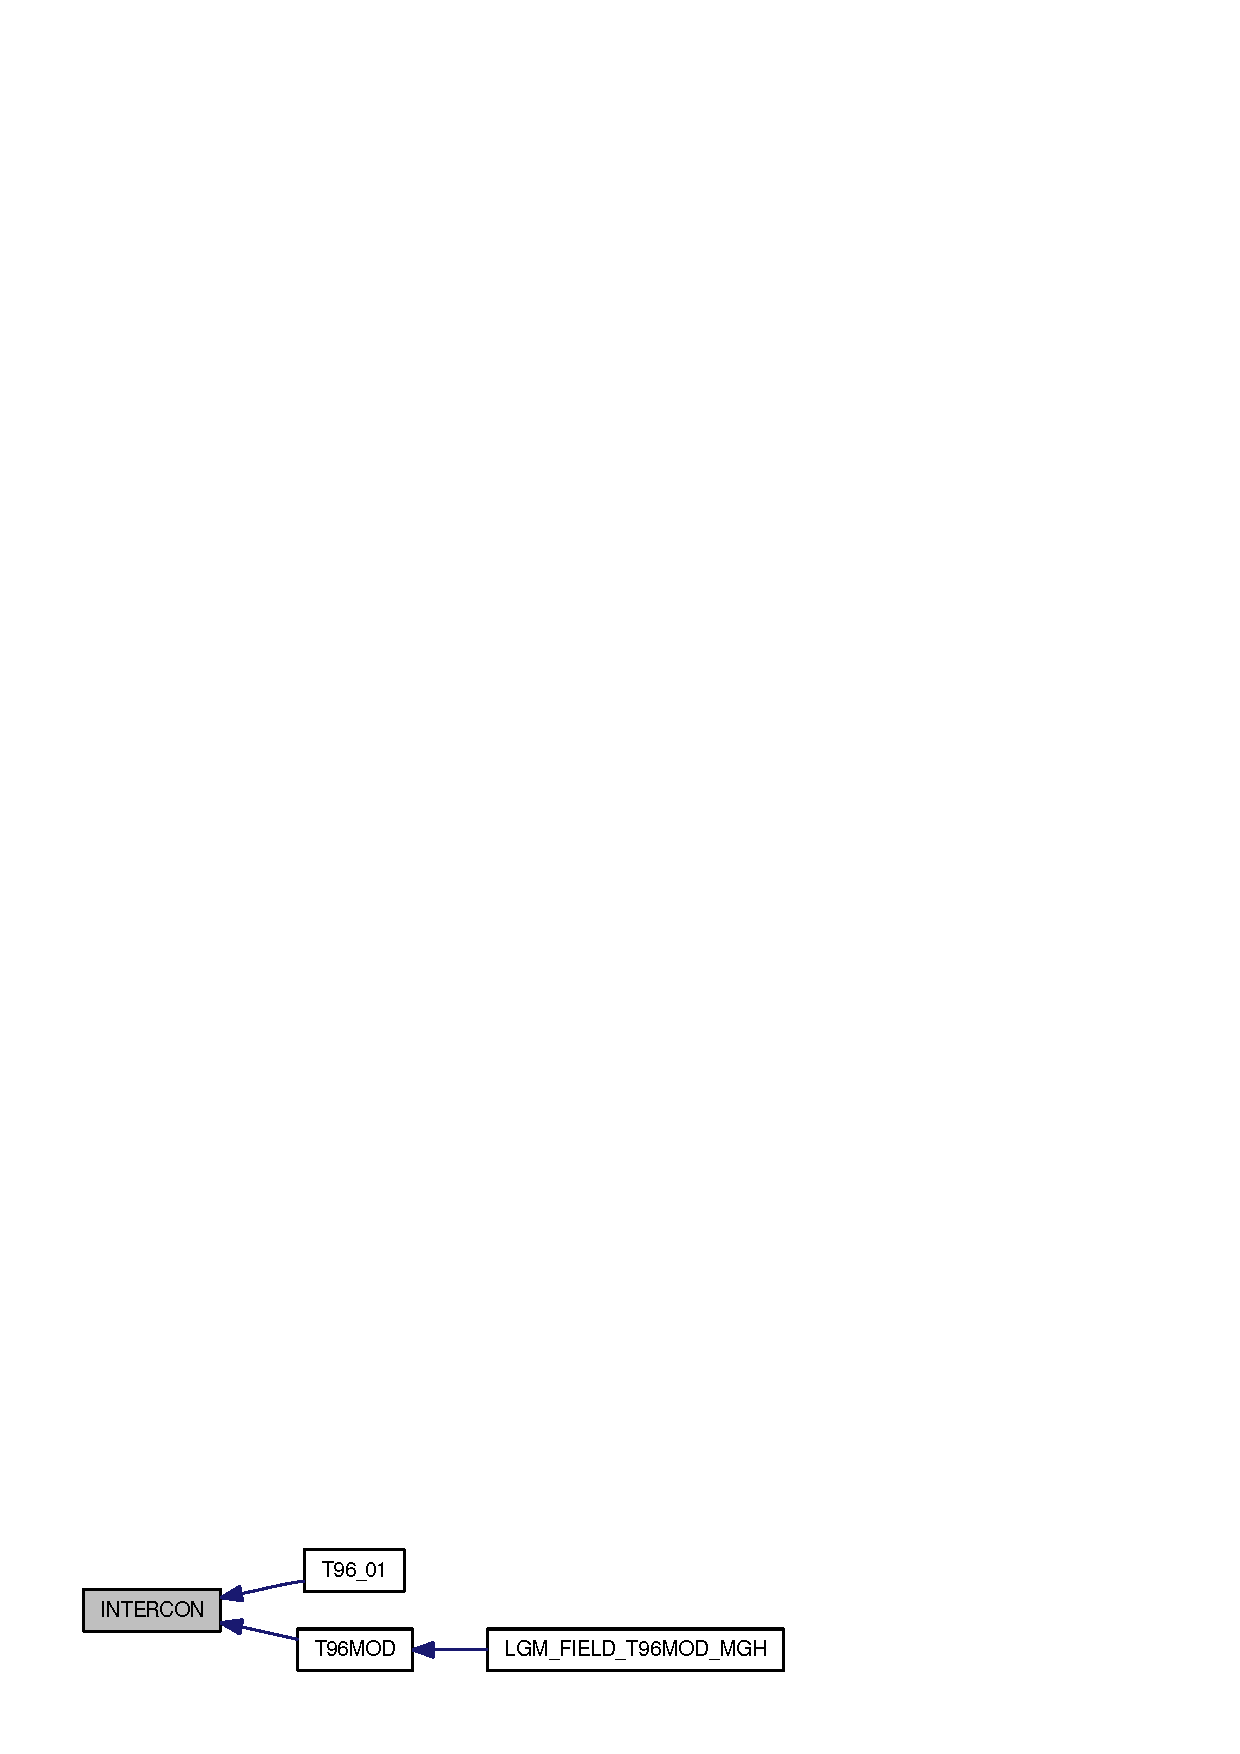
\includegraphics[width=190pt]{_t96mod_8f_2e097fa1f961156bc2ca8b94983b9e4f_icgraph}
\end{center}
\end{figure}
\hypertarget{_t96mod_8f_a2c7e086277c827ff05f4a9c6eb99b2b}{
\index{T96mod.f@{T96mod.f}!TAILRC96@{TAILRC96}}
\index{TAILRC96@{TAILRC96}!T96mod.f@{T96mod.f}}
\subsubsection[{TAILRC96}]{\setlength{\rightskip}{0pt plus 5cm}subroutine TAILRC96 (DMODIF, \/  SPS, \/  X, \/  Y, \/  Z, \/  BXRC, \/  BYRC, \/  BZRC, \/  BXT2, \/  BYT2, \/  $\ast$ {\em BZT2}, \/  BXT3, \/  BYT3, \/  BZT3, \/  BXT2ADD, \/  BYT2ADD, \/  BZT2ADD)}}
\label{_t96mod_8f_a2c7e086277c827ff05f4a9c6eb99b2b}




Definition at line 744 of file T96mod.f.

Here is the call graph for this function:\nopagebreak
\begin{figure}[H]
\begin{center}
\leavevmode
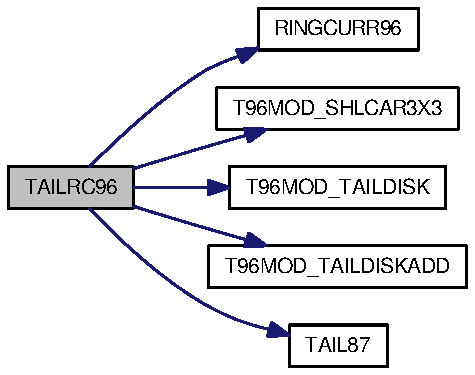
\includegraphics[width=132pt]{_t96mod_8f_a2c7e086277c827ff05f4a9c6eb99b2b_cgraph}
\end{center}
\end{figure}


Here is the caller graph for this function:\nopagebreak
\begin{figure}[H]
\begin{center}
\leavevmode
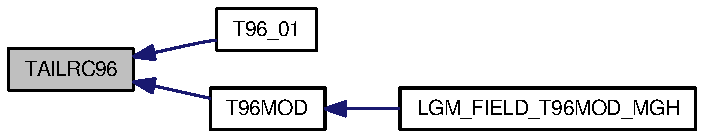
\includegraphics[width=187pt]{_t96mod_8f_a2c7e086277c827ff05f4a9c6eb99b2b_icgraph}
\end{center}
\end{figure}
\hypertarget{_t96mod_8f_87fae8404610c1e792fff8db728b60a3}{
\index{T96mod.f@{T96mod.f}!RINGCURR96@{RINGCURR96}}
\index{RINGCURR96@{RINGCURR96}!T96mod.f@{T96mod.f}}
\subsubsection[{RINGCURR96}]{\setlength{\rightskip}{0pt plus 5cm}subroutine RINGCURR96 (X, \/  Y, \/  Z, \/  BX, \/  BY, \/  BZ)}}
\label{_t96mod_8f_87fae8404610c1e792fff8db728b60a3}




Definition at line 872 of file T96mod.f.

Here is the caller graph for this function:\nopagebreak
\begin{figure}[H]
\begin{center}
\leavevmode
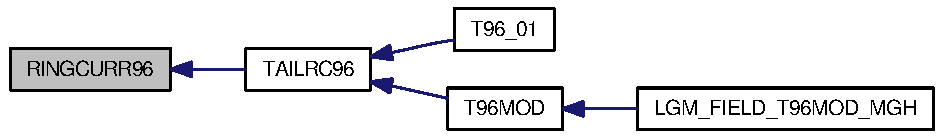
\includegraphics[width=244pt]{_t96mod_8f_87fae8404610c1e792fff8db728b60a3_icgraph}
\end{center}
\end{figure}
\hypertarget{_t96mod_8f_b0a52ce0e8651f818014bb9cd0040927}{
\index{T96mod.f@{T96mod.f}!T96MOD\_\-TAILDISK@{T96MOD\_\-TAILDISK}}
\index{T96MOD\_\-TAILDISK@{T96MOD\_\-TAILDISK}!T96mod.f@{T96mod.f}}
\subsubsection[{T96MOD\_\-TAILDISK}]{\setlength{\rightskip}{0pt plus 5cm}subroutine T96MOD\_\-TAILDISK (X, \/  Y, \/  Z, \/  BX, \/  BY, \/  BZ)}}
\label{_t96mod_8f_b0a52ce0e8651f818014bb9cd0040927}




Definition at line 974 of file T96mod.f.

Here is the caller graph for this function:\nopagebreak
\begin{figure}[H]
\begin{center}
\leavevmode
\includegraphics[width=257pt]{_t96mod_8f_b0a52ce0e8651f818014bb9cd0040927_icgraph}
\end{center}
\end{figure}
\hypertarget{_t96mod_8f_cbb331c88d418399755655497d909b64}{
\index{T96mod.f@{T96mod.f}!T96MOD\_\-TAILDISKADD@{T96MOD\_\-TAILDISKADD}}
\index{T96MOD\_\-TAILDISKADD@{T96MOD\_\-TAILDISKADD}!T96mod.f@{T96mod.f}}
\subsubsection[{T96MOD\_\-TAILDISKADD}]{\setlength{\rightskip}{0pt plus 5cm}subroutine T96MOD\_\-TAILDISKADD (DMODIF, \/  X, \/  Y, \/  Z, \/  BX, \/  BY, \/  BZ)}}
\label{_t96mod_8f_cbb331c88d418399755655497d909b64}




Definition at line 1063 of file T96mod.f.

Here is the caller graph for this function:\nopagebreak
\begin{figure}[H]
\begin{center}
\leavevmode
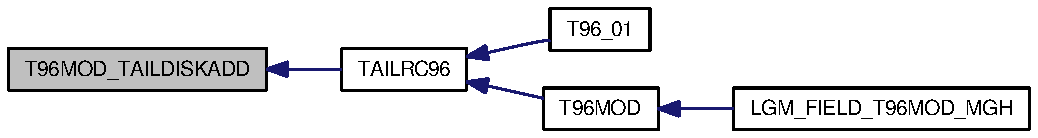
\includegraphics[width=267pt]{_t96mod_8f_cbb331c88d418399755655497d909b64_icgraph}
\end{center}
\end{figure}
\hypertarget{_t96mod_8f_f7a0147645dfe77e8197e10963ed3770}{
\index{T96mod.f@{T96mod.f}!TAIL87@{TAIL87}}
\index{TAIL87@{TAIL87}!T96mod.f@{T96mod.f}}
\subsubsection[{TAIL87}]{\setlength{\rightskip}{0pt plus 5cm}subroutine TAIL87 (X, \/  Z, \/  BX, \/  BZ)}}
\label{_t96mod_8f_f7a0147645dfe77e8197e10963ed3770}




Definition at line 1163 of file T96mod.f.

Here is the caller graph for this function:\nopagebreak
\begin{figure}[H]
\begin{center}
\leavevmode
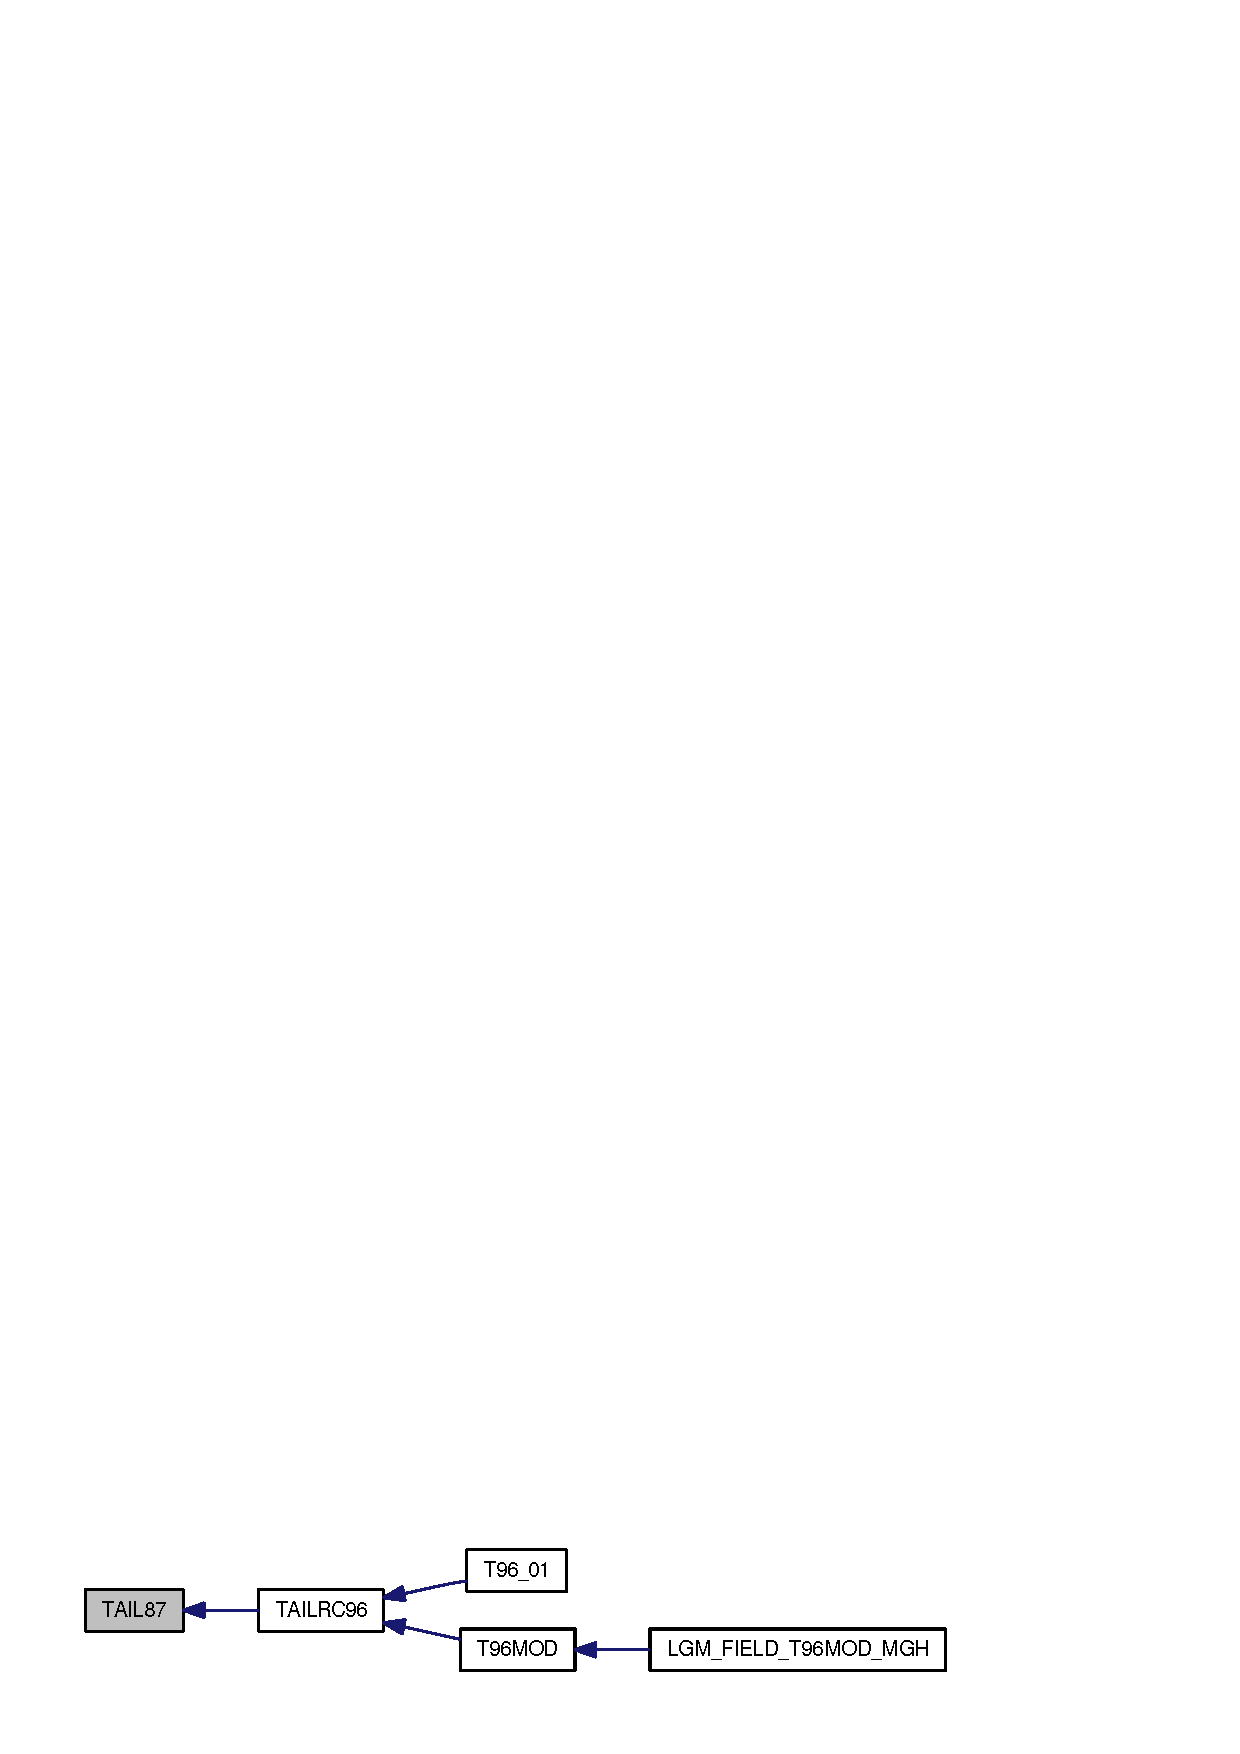
\includegraphics[width=229pt]{_t96mod_8f_f7a0147645dfe77e8197e10963ed3770_icgraph}
\end{center}
\end{figure}
\hypertarget{_t96mod_8f_0918ae2ac8568570f93f2d5c0d88f9dc}{
\index{T96mod.f@{T96mod.f}!T96MOD\_\-SHLCAR3X3@{T96MOD\_\-SHLCAR3X3}}
\index{T96MOD\_\-SHLCAR3X3@{T96MOD\_\-SHLCAR3X3}!T96mod.f@{T96mod.f}}
\subsubsection[{T96MOD\_\-SHLCAR3X3}]{\setlength{\rightskip}{0pt plus 5cm}subroutine T96MOD\_\-SHLCAR3X3 (A, \/  X, \/  Y, \/  Z, \/  SPS, \/  HX, \/  HY, \/  HZ)}}
\label{_t96mod_8f_0918ae2ac8568570f93f2d5c0d88f9dc}




Definition at line 1284 of file T96mod.f.

Here is the caller graph for this function:\nopagebreak
\begin{figure}[H]
\begin{center}
\leavevmode
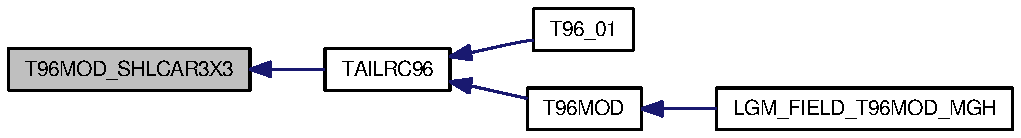
\includegraphics[width=263pt]{_t96mod_8f_0918ae2ac8568570f93f2d5c0d88f9dc_icgraph}
\end{center}
\end{figure}
\hypertarget{_t96mod_8f_1d35065857c1597a4d45699d6e30faa9}{
\index{T96mod.f@{T96mod.f}!BIRK1TOT\_\-02@{BIRK1TOT\_\-02}}
\index{BIRK1TOT\_\-02@{BIRK1TOT\_\-02}!T96mod.f@{T96mod.f}}
\subsubsection[{BIRK1TOT\_\-02}]{\setlength{\rightskip}{0pt plus 5cm}subroutine BIRK1TOT\_\-02 (PS, \/  X, \/  Y, \/  Z, \/  BX, \/  BY, \/  BZ)}}
\label{_t96mod_8f_1d35065857c1597a4d45699d6e30faa9}




Definition at line 1377 of file T96mod.f.

Here is the call graph for this function:\nopagebreak
\begin{figure}[H]
\begin{center}
\leavevmode
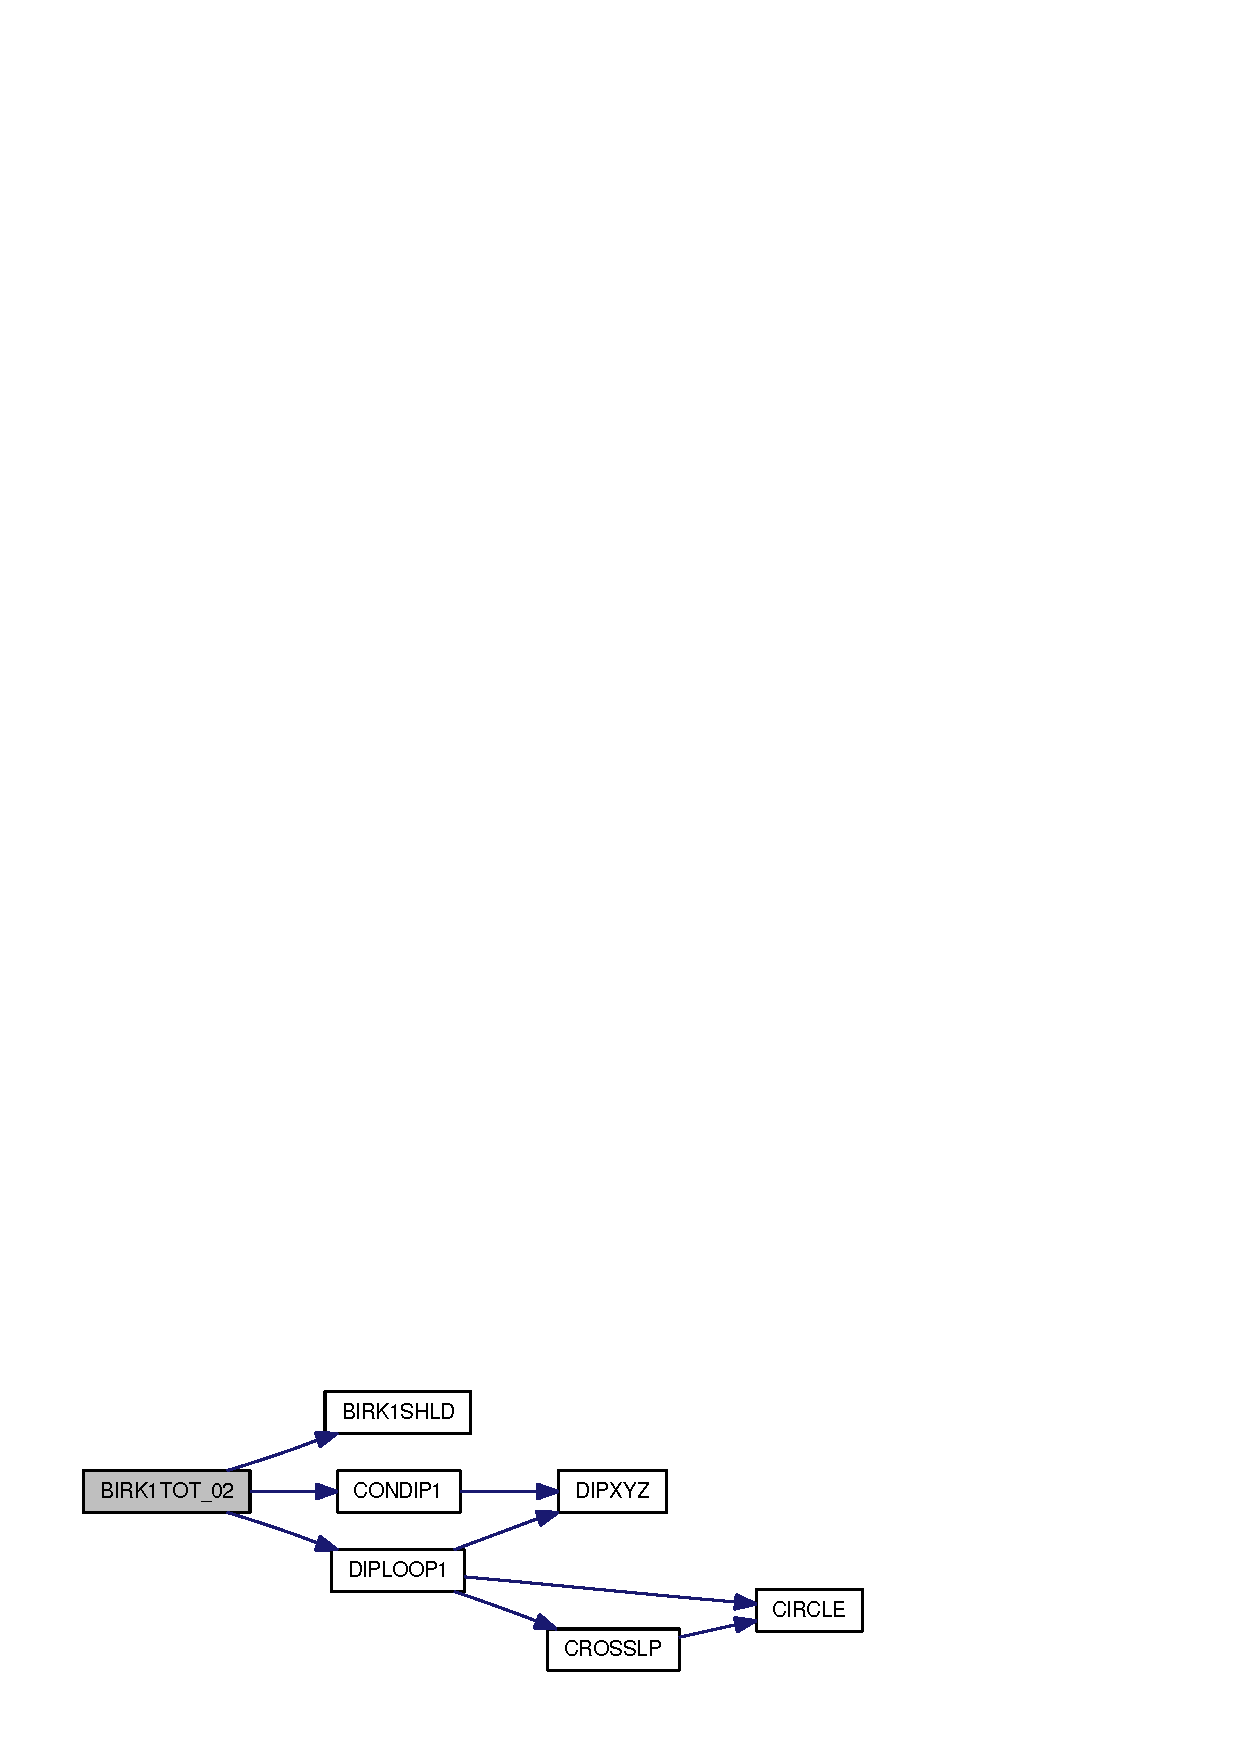
\includegraphics[width=209pt]{_t96mod_8f_1d35065857c1597a4d45699d6e30faa9_cgraph}
\end{center}
\end{figure}


Here is the caller graph for this function:\nopagebreak
\begin{figure}[H]
\begin{center}
\leavevmode
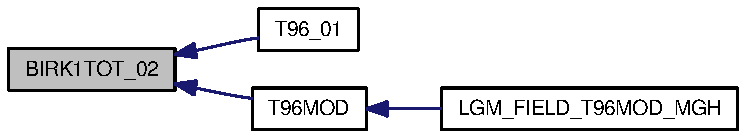
\includegraphics[width=197pt]{_t96mod_8f_1d35065857c1597a4d45699d6e30faa9_icgraph}
\end{center}
\end{figure}
\hypertarget{_t96mod_8f_7634ccf219c90ebc36de1b55b961ed88}{
\index{T96mod.f@{T96mod.f}!DIPLOOP1@{DIPLOOP1}}
\index{DIPLOOP1@{DIPLOOP1}!T96mod.f@{T96mod.f}}
\subsubsection[{DIPLOOP1}]{\setlength{\rightskip}{0pt plus 5cm}subroutine DIPLOOP1 (XI, \/  D)}}
\label{_t96mod_8f_7634ccf219c90ebc36de1b55b961ed88}




Definition at line 1652 of file T96mod.f.

Here is the call graph for this function:\nopagebreak
\begin{figure}[H]
\begin{center}
\leavevmode
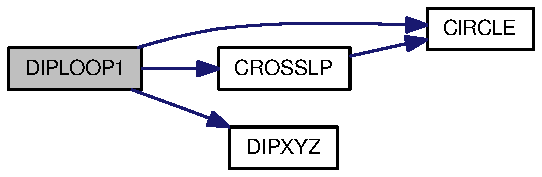
\includegraphics[width=148pt]{_t96mod_8f_7634ccf219c90ebc36de1b55b961ed88_cgraph}
\end{center}
\end{figure}


Here is the caller graph for this function:\nopagebreak
\begin{figure}[H]
\begin{center}
\leavevmode
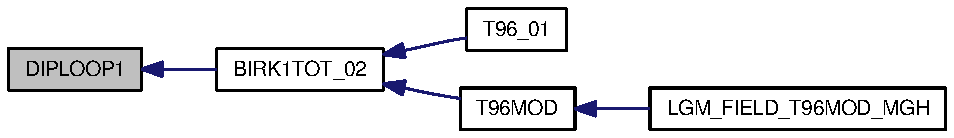
\includegraphics[width=247pt]{_t96mod_8f_7634ccf219c90ebc36de1b55b961ed88_icgraph}
\end{center}
\end{figure}
\hypertarget{_t96mod_8f_7ad3cc17a6906d0de0ea87905c8adfa0}{
\index{T96mod.f@{T96mod.f}!CIRCLE@{CIRCLE}}
\index{CIRCLE@{CIRCLE}!T96mod.f@{T96mod.f}}
\subsubsection[{CIRCLE}]{\setlength{\rightskip}{0pt plus 5cm}subroutine CIRCLE (X, \/  Y, \/  Z, \/  RL, \/  BX, \/  BY, \/  BZ)}}
\label{_t96mod_8f_7ad3cc17a6906d0de0ea87905c8adfa0}




Definition at line 1771 of file T96mod.f.

Here is the caller graph for this function:\nopagebreak
\begin{figure}[H]
\begin{center}
\leavevmode
\includegraphics[width=388pt]{_t96mod_8f_7ad3cc17a6906d0de0ea87905c8adfa0_icgraph}
\end{center}
\end{figure}
\hypertarget{_t96mod_8f_339de23a7fc16677d5c934050601456b}{
\index{T96mod.f@{T96mod.f}!CROSSLP@{CROSSLP}}
\index{CROSSLP@{CROSSLP}!T96mod.f@{T96mod.f}}
\subsubsection[{CROSSLP}]{\setlength{\rightskip}{0pt plus 5cm}subroutine CROSSLP (X, \/  Y, \/  Z, \/  BX, \/  BY, \/  BZ, \/  XC, \/  RL, \/  AL)}}
\label{_t96mod_8f_339de23a7fc16677d5c934050601456b}




Definition at line 1811 of file T96mod.f.

Here is the call graph for this function:\nopagebreak
\begin{figure}[H]
\begin{center}
\leavevmode
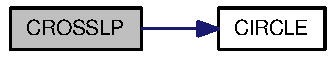
\includegraphics[width=98pt]{_t96mod_8f_339de23a7fc16677d5c934050601456b_cgraph}
\end{center}
\end{figure}


Here is the caller graph for this function:\nopagebreak
\begin{figure}[H]
\begin{center}
\leavevmode
\includegraphics[width=344pt]{_t96mod_8f_339de23a7fc16677d5c934050601456b_icgraph}
\end{center}
\end{figure}
\hypertarget{_t96mod_8f_76f3ffff48346c7a53f738f013945222}{
\index{T96mod.f@{T96mod.f}!DIPXYZ@{DIPXYZ}}
\index{DIPXYZ@{DIPXYZ}!T96mod.f@{T96mod.f}}
\subsubsection[{DIPXYZ}]{\setlength{\rightskip}{0pt plus 5cm}subroutine DIPXYZ (X, \/  Y, \/  Z, \/  BXX, \/  BYX, \/  BZX, \/  BXY, \/  BYY, \/  BZY, \/  BXZ, \/  BYZ, \/  BZZ)}}
\label{_t96mod_8f_76f3ffff48346c7a53f738f013945222}




Definition at line 1838 of file T96mod.f.

Here is the caller graph for this function:\nopagebreak
\begin{figure}[H]
\begin{center}
\leavevmode
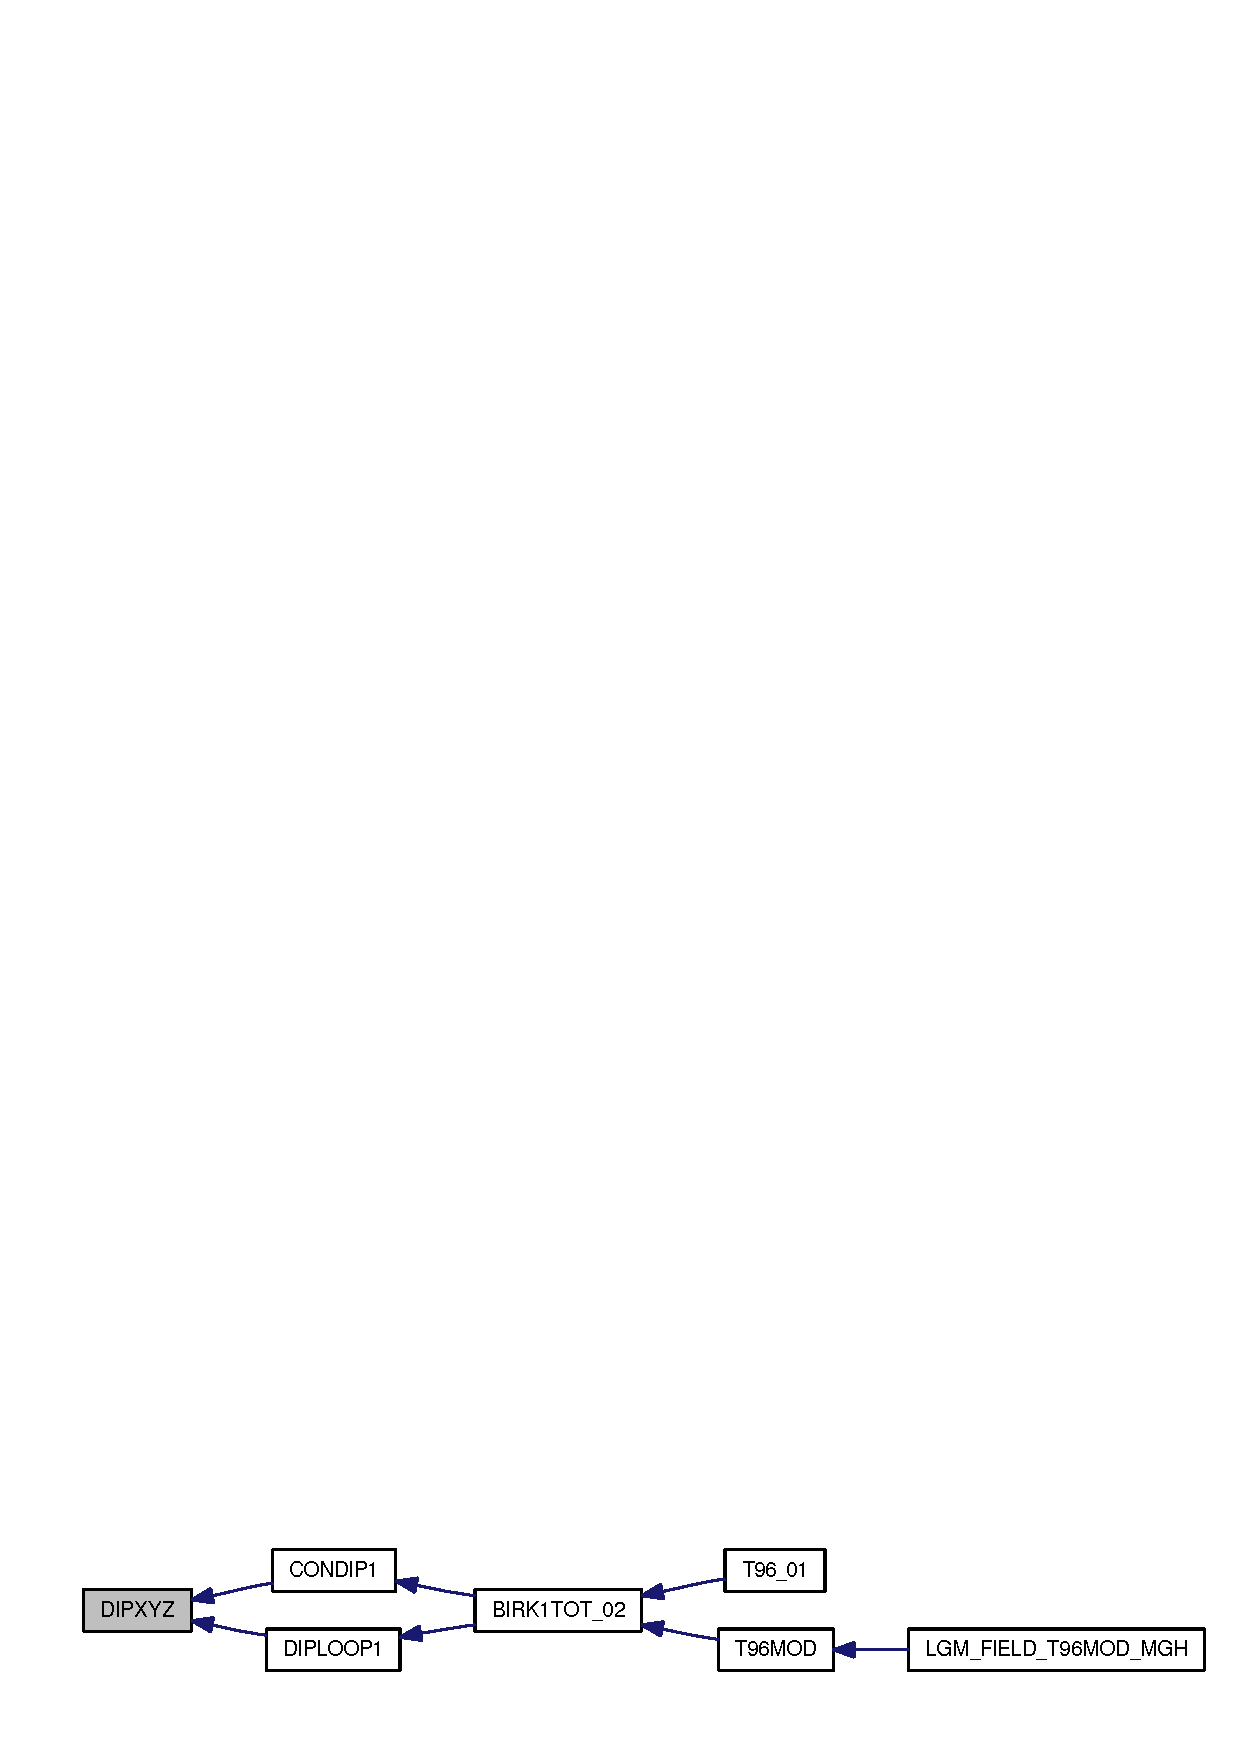
\includegraphics[width=291pt]{_t96mod_8f_76f3ffff48346c7a53f738f013945222_icgraph}
\end{center}
\end{figure}
\hypertarget{_t96mod_8f_2432dab29def6a7f82b4e61542784ca2}{
\index{T96mod.f@{T96mod.f}!CONDIP1@{CONDIP1}}
\index{CONDIP1@{CONDIP1}!T96mod.f@{T96mod.f}}
\subsubsection[{CONDIP1}]{\setlength{\rightskip}{0pt plus 5cm}subroutine CONDIP1 (XI, \/  D)}}
\label{_t96mod_8f_2432dab29def6a7f82b4e61542784ca2}




Definition at line 1868 of file T96mod.f.

Here is the call graph for this function:\nopagebreak
\begin{figure}[H]
\begin{center}
\leavevmode
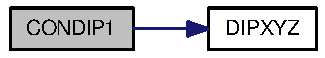
\includegraphics[width=96pt]{_t96mod_8f_2432dab29def6a7f82b4e61542784ca2_cgraph}
\end{center}
\end{figure}


Here is the caller graph for this function:\nopagebreak
\begin{figure}[H]
\begin{center}
\leavevmode
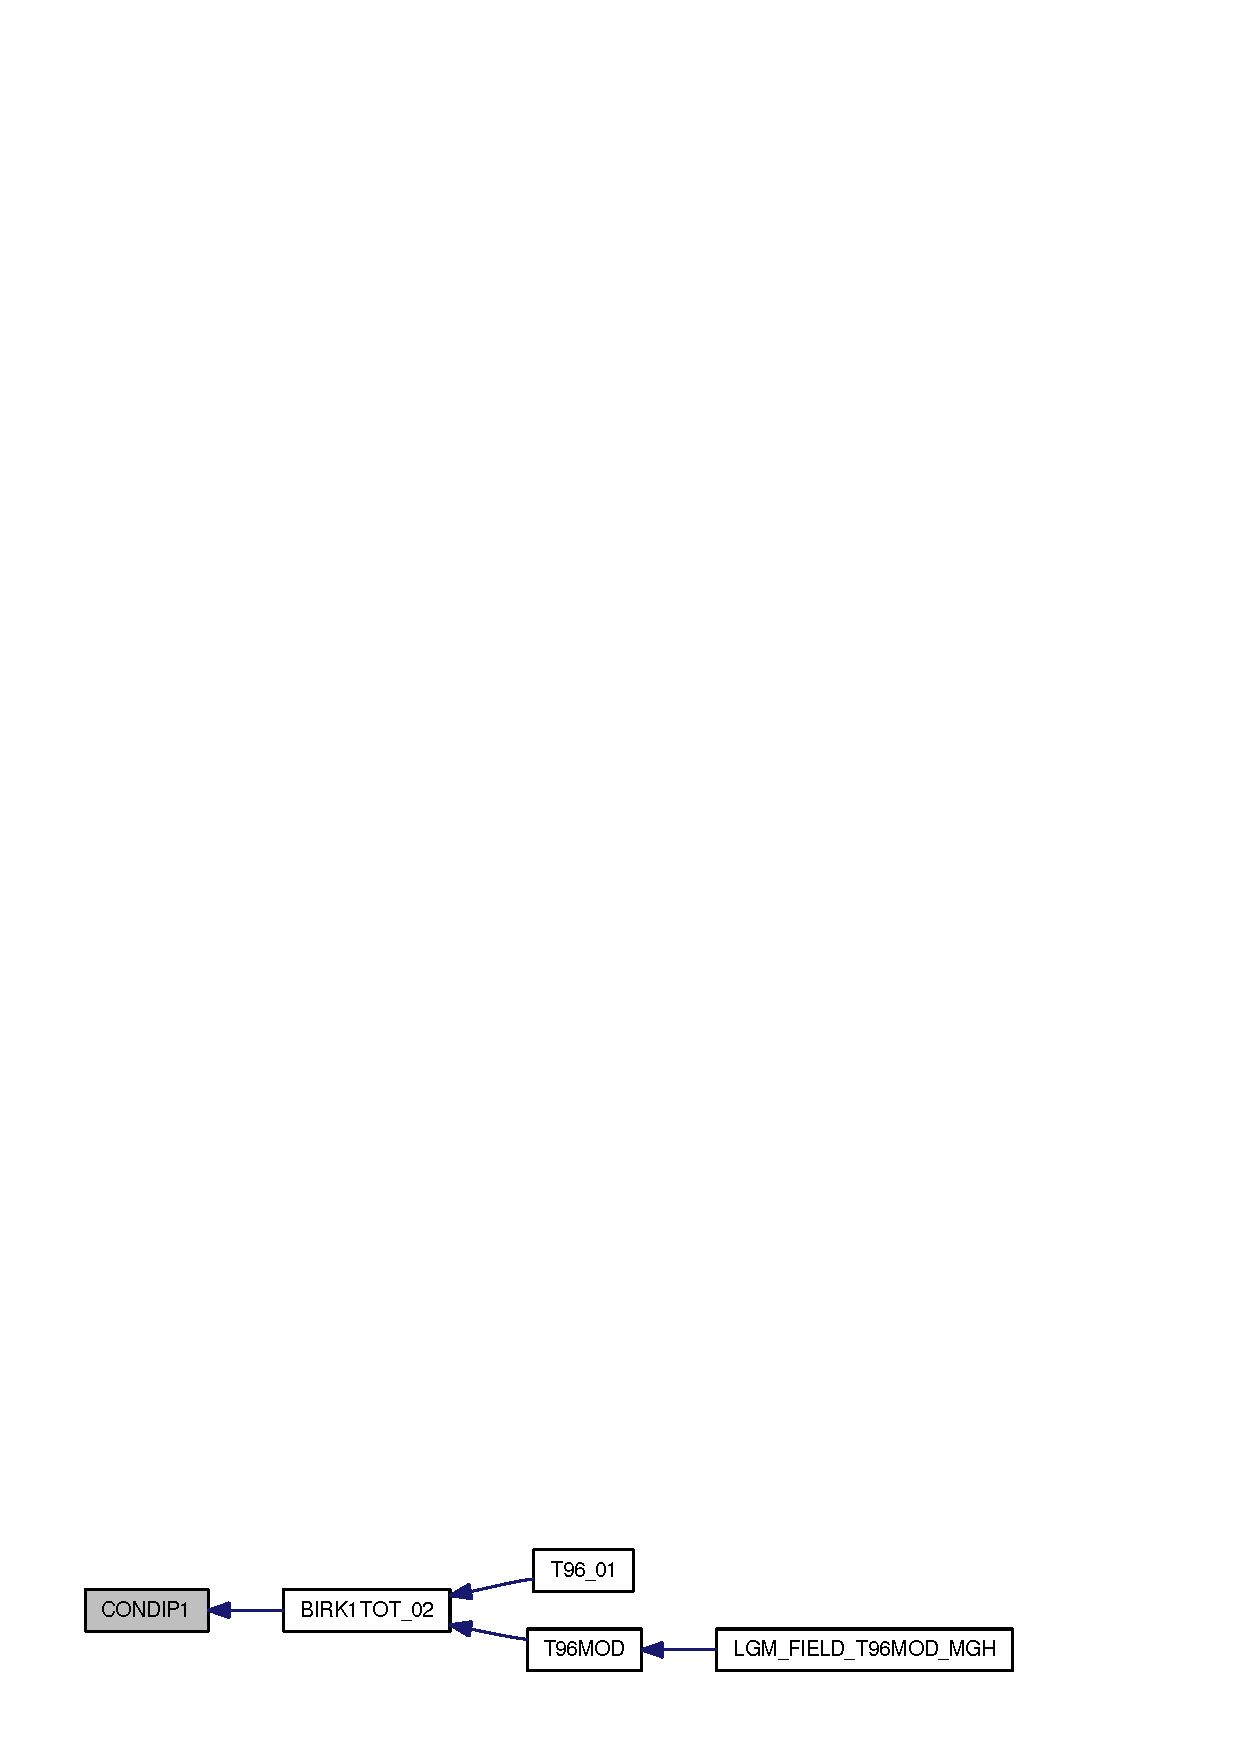
\includegraphics[width=245pt]{_t96mod_8f_2432dab29def6a7f82b4e61542784ca2_icgraph}
\end{center}
\end{figure}
\hypertarget{_t96mod_8f_e7df392ea162336df5811079016b08ac}{
\index{T96mod.f@{T96mod.f}!BIRK1SHLD@{BIRK1SHLD}}
\index{BIRK1SHLD@{BIRK1SHLD}!T96mod.f@{T96mod.f}}
\subsubsection[{BIRK1SHLD}]{\setlength{\rightskip}{0pt plus 5cm}subroutine BIRK1SHLD (PS, \/  X, \/  Y, \/  Z, \/  BX, \/  BY, \/  BZ)}}
\label{_t96mod_8f_e7df392ea162336df5811079016b08ac}




Definition at line 2028 of file T96mod.f.

Here is the caller graph for this function:\nopagebreak
\begin{figure}[H]
\begin{center}
\leavevmode
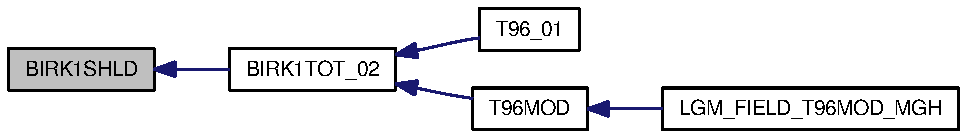
\includegraphics[width=250pt]{_t96mod_8f_e7df392ea162336df5811079016b08ac_icgraph}
\end{center}
\end{figure}
\hypertarget{_t96mod_8f_72d9123c4c7f8cc57e525a533b45d5fe}{
\index{T96mod.f@{T96mod.f}!BIRK2TOT\_\-02@{BIRK2TOT\_\-02}}
\index{BIRK2TOT\_\-02@{BIRK2TOT\_\-02}!T96mod.f@{T96mod.f}}
\subsubsection[{BIRK2TOT\_\-02}]{\setlength{\rightskip}{0pt plus 5cm}subroutine BIRK2TOT\_\-02 (PS, \/  X, \/  Y, \/  Z, \/  BX, \/  BY, \/  BZ)}}
\label{_t96mod_8f_72d9123c4c7f8cc57e525a533b45d5fe}




Definition at line 2135 of file T96mod.f.

Here is the call graph for this function:\nopagebreak
\begin{figure}[H]
\begin{center}
\leavevmode
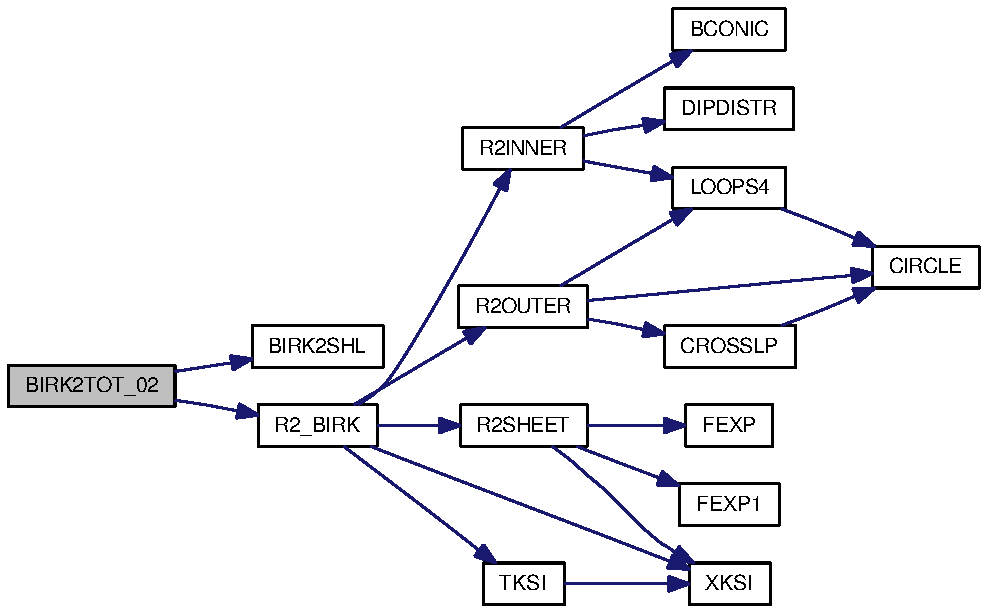
\includegraphics[width=255pt]{_t96mod_8f_72d9123c4c7f8cc57e525a533b45d5fe_cgraph}
\end{center}
\end{figure}


Here is the caller graph for this function:\nopagebreak
\begin{figure}[H]
\begin{center}
\leavevmode
\includegraphics[width=197pt]{_t96mod_8f_72d9123c4c7f8cc57e525a533b45d5fe_icgraph}
\end{center}
\end{figure}
\hypertarget{_t96mod_8f_09ee39e02874a680b5fe915e9ccbc8f6}{
\index{T96mod.f@{T96mod.f}!BIRK2SHL@{BIRK2SHL}}
\index{BIRK2SHL@{BIRK2SHL}!T96mod.f@{T96mod.f}}
\subsubsection[{BIRK2SHL}]{\setlength{\rightskip}{0pt plus 5cm}subroutine BIRK2SHL (X, \/  Y, \/  Z, \/  PS, \/  HX, \/  HY, \/  HZ)}}
\label{_t96mod_8f_09ee39e02874a680b5fe915e9ccbc8f6}




Definition at line 2151 of file T96mod.f.

Here is the caller graph for this function:\nopagebreak
\begin{figure}[H]
\begin{center}
\leavevmode
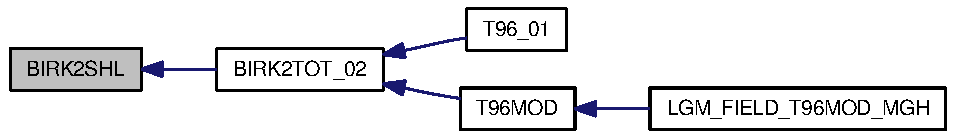
\includegraphics[width=247pt]{_t96mod_8f_09ee39e02874a680b5fe915e9ccbc8f6_icgraph}
\end{center}
\end{figure}
\hypertarget{_t96mod_8f_75644447b8b698b1ea33e1bc67aba7af}{
\index{T96mod.f@{T96mod.f}!R2\_\-BIRK@{R2\_\-BIRK}}
\index{R2\_\-BIRK@{R2\_\-BIRK}!T96mod.f@{T96mod.f}}
\subsubsection[{R2\_\-BIRK}]{\setlength{\rightskip}{0pt plus 5cm}subroutine R2\_\-BIRK (X, \/  Y, \/  Z, \/  PS, \/  BX, \/  BY, \/  BZ)}}
\label{_t96mod_8f_75644447b8b698b1ea33e1bc67aba7af}




Definition at line 2249 of file T96mod.f.

Here is the call graph for this function:\nopagebreak
\begin{figure}[H]
\begin{center}
\leavevmode
\includegraphics[width=194pt]{_t96mod_8f_75644447b8b698b1ea33e1bc67aba7af_cgraph}
\end{center}
\end{figure}


Here is the caller graph for this function:\nopagebreak
\begin{figure}[H]
\begin{center}
\leavevmode
\includegraphics[width=244pt]{_t96mod_8f_75644447b8b698b1ea33e1bc67aba7af_icgraph}
\end{center}
\end{figure}
\hypertarget{_t96mod_8f_717e6c5b669e682bef3f33b1a4a73796}{
\index{T96mod.f@{T96mod.f}!R2INNER@{R2INNER}}
\index{R2INNER@{R2INNER}!T96mod.f@{T96mod.f}}
\subsubsection[{R2INNER}]{\setlength{\rightskip}{0pt plus 5cm}subroutine R2INNER (X, \/  Y, \/  Z, \/  BX, \/  BY, \/  BZ)}}
\label{_t96mod_8f_717e6c5b669e682bef3f33b1a4a73796}




Definition at line 2315 of file T96mod.f.

Here is the call graph for this function:\nopagebreak
\begin{figure}[H]
\begin{center}
\leavevmode
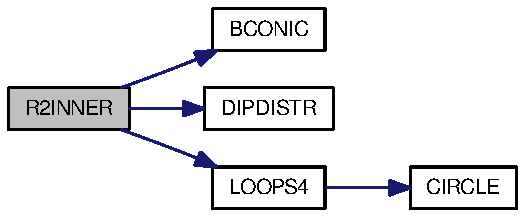
\includegraphics[width=144pt]{_t96mod_8f_717e6c5b669e682bef3f33b1a4a73796_cgraph}
\end{center}
\end{figure}


Here is the caller graph for this function:\nopagebreak
\begin{figure}[H]
\begin{center}
\leavevmode
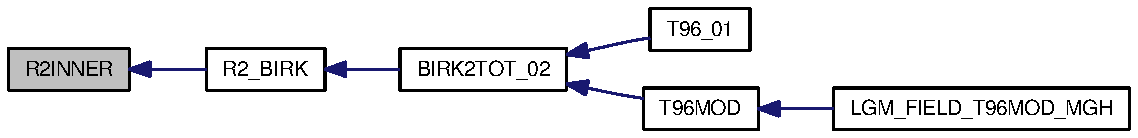
\includegraphics[width=291pt]{_t96mod_8f_717e6c5b669e682bef3f33b1a4a73796_icgraph}
\end{center}
\end{figure}
\hypertarget{_t96mod_8f_1a6fae1af90cf34b2b4e95d5ecde87a9}{
\index{T96mod.f@{T96mod.f}!BCONIC@{BCONIC}}
\index{BCONIC@{BCONIC}!T96mod.f@{T96mod.f}}
\subsubsection[{BCONIC}]{\setlength{\rightskip}{0pt plus 5cm}subroutine BCONIC (X, \/  Y, \/  Z, \/  CBX, \/  CBY, \/  CBZ, \/  NMAX)}}
\label{_t96mod_8f_1a6fae1af90cf34b2b4e95d5ecde87a9}




Definition at line 2348 of file T96mod.f.

Here is the caller graph for this function:\nopagebreak
\begin{figure}[H]
\begin{center}
\leavevmode
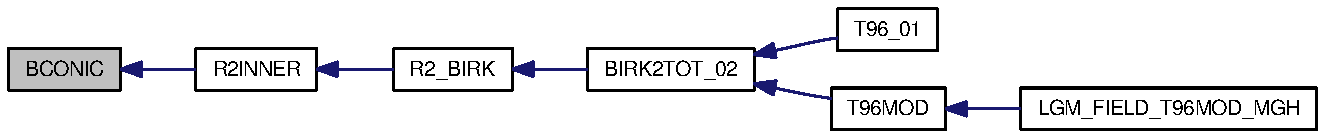
\includegraphics[width=336pt]{_t96mod_8f_1a6fae1af90cf34b2b4e95d5ecde87a9_icgraph}
\end{center}
\end{figure}
\hypertarget{_t96mod_8f_26863a8d653e16bfa831cf1cd3d57367}{
\index{T96mod.f@{T96mod.f}!DIPDISTR@{DIPDISTR}}
\index{DIPDISTR@{DIPDISTR}!T96mod.f@{T96mod.f}}
\subsubsection[{DIPDISTR}]{\setlength{\rightskip}{0pt plus 5cm}subroutine DIPDISTR (X, \/  Y, \/  Z, \/  BX, \/  BY, \/  BZ, \/  MODE)}}
\label{_t96mod_8f_26863a8d653e16bfa831cf1cd3d57367}




Definition at line 2395 of file T96mod.f.

Here is the caller graph for this function:\nopagebreak
\begin{figure}[H]
\begin{center}
\leavevmode
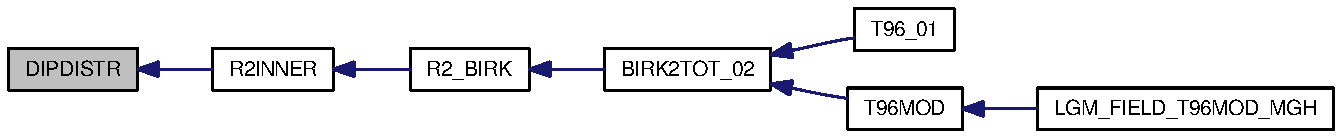
\includegraphics[width=340pt]{_t96mod_8f_26863a8d653e16bfa831cf1cd3d57367_icgraph}
\end{center}
\end{figure}
\hypertarget{_t96mod_8f_4b792e262830f77251236192fe6ade49}{
\index{T96mod.f@{T96mod.f}!R2OUTER@{R2OUTER}}
\index{R2OUTER@{R2OUTER}!T96mod.f@{T96mod.f}}
\subsubsection[{R2OUTER}]{\setlength{\rightskip}{0pt plus 5cm}subroutine R2OUTER (X, \/  Y, \/  Z, \/  BX, \/  BY, \/  BZ)}}
\label{_t96mod_8f_4b792e262830f77251236192fe6ade49}




Definition at line 2427 of file T96mod.f.

Here is the call graph for this function:\nopagebreak
\begin{figure}[H]
\begin{center}
\leavevmode
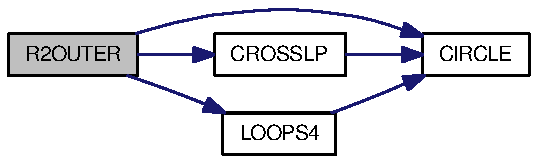
\includegraphics[width=147pt]{_t96mod_8f_4b792e262830f77251236192fe6ade49_cgraph}
\end{center}
\end{figure}


Here is the caller graph for this function:\nopagebreak
\begin{figure}[H]
\begin{center}
\leavevmode
\includegraphics[width=293pt]{_t96mod_8f_4b792e262830f77251236192fe6ade49_icgraph}
\end{center}
\end{figure}
\hypertarget{_t96mod_8f_8bb46e1322b561a6e5aa91de2b85a0e2}{
\index{T96mod.f@{T96mod.f}!LOOPS4@{LOOPS4}}
\index{LOOPS4@{LOOPS4}!T96mod.f@{T96mod.f}}
\subsubsection[{LOOPS4}]{\setlength{\rightskip}{0pt plus 5cm}subroutine LOOPS4 (X, \/  Y, \/  Z, \/  BX, \/  BY, \/  BZ, \/  XC, \/  YC, \/  ZC, \/  R, \/  THETA, \/  PHI)}}
\label{_t96mod_8f_8bb46e1322b561a6e5aa91de2b85a0e2}




Definition at line 2464 of file T96mod.f.

Here is the call graph for this function:\nopagebreak
\begin{figure}[H]
\begin{center}
\leavevmode
\includegraphics[width=93pt]{_t96mod_8f_8bb46e1322b561a6e5aa91de2b85a0e2_cgraph}
\end{center}
\end{figure}


Here is the caller graph for this function:\nopagebreak
\begin{figure}[H]
\begin{center}
\leavevmode
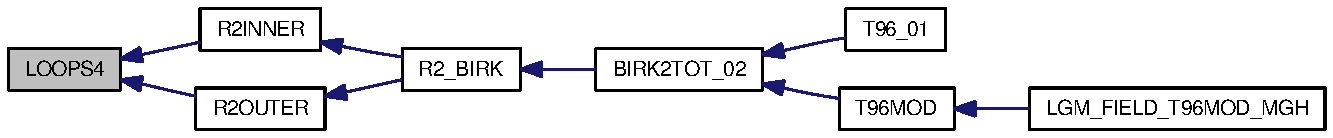
\includegraphics[width=338pt]{_t96mod_8f_8bb46e1322b561a6e5aa91de2b85a0e2_icgraph}
\end{center}
\end{figure}
\hypertarget{_t96mod_8f_d2c23a8a964ae249deaa1665da76803f}{
\index{T96mod.f@{T96mod.f}!R2SHEET@{R2SHEET}}
\index{R2SHEET@{R2SHEET}!T96mod.f@{T96mod.f}}
\subsubsection[{R2SHEET}]{\setlength{\rightskip}{0pt plus 5cm}subroutine R2SHEET (X, \/  Y, \/  Z, \/  BX, \/  BY, \/  BZ)}}
\label{_t96mod_8f_d2c23a8a964ae249deaa1665da76803f}




Definition at line 2540 of file T96mod.f.

Here is the call graph for this function:\nopagebreak
\begin{figure}[H]
\begin{center}
\leavevmode
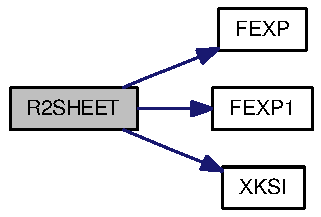
\includegraphics[width=95pt]{_t96mod_8f_d2c23a8a964ae249deaa1665da76803f_cgraph}
\end{center}
\end{figure}


Here is the caller graph for this function:\nopagebreak
\begin{figure}[H]
\begin{center}
\leavevmode
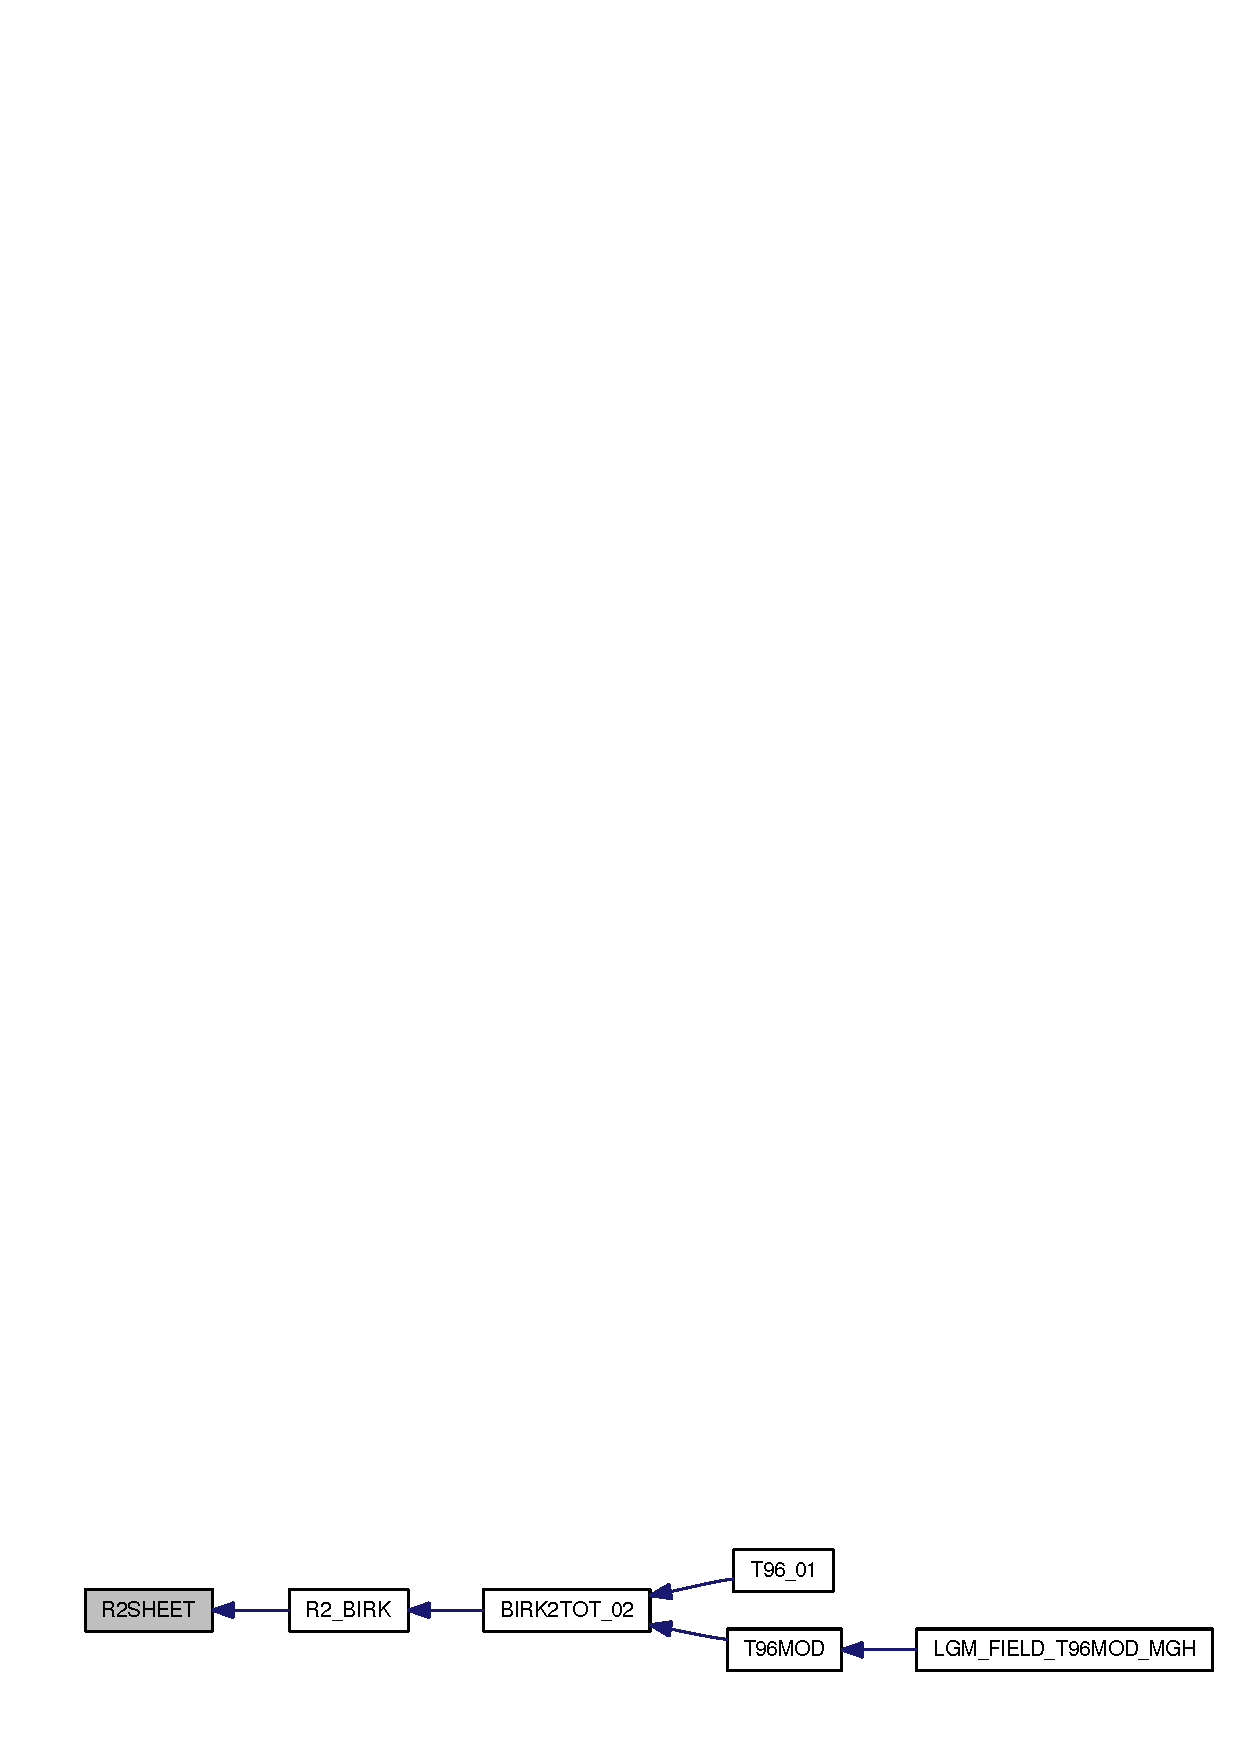
\includegraphics[width=293pt]{_t96mod_8f_d2c23a8a964ae249deaa1665da76803f_icgraph}
\end{center}
\end{figure}
\hypertarget{_t96mod_8f_34df9615369af608c58c50830a71bc2c}{
\index{T96mod.f@{T96mod.f}!XKSI@{XKSI}}
\index{XKSI@{XKSI}!T96mod.f@{T96mod.f}}
\subsubsection[{XKSI}]{\setlength{\rightskip}{0pt plus 5cm}DOUBLE PRECISION XKSI (X, \/  Y, \/  Z)}}
\label{_t96mod_8f_34df9615369af608c58c50830a71bc2c}




Definition at line 2734 of file T96mod.f.

Here is the caller graph for this function:\nopagebreak
\begin{figure}[H]
\begin{center}
\leavevmode
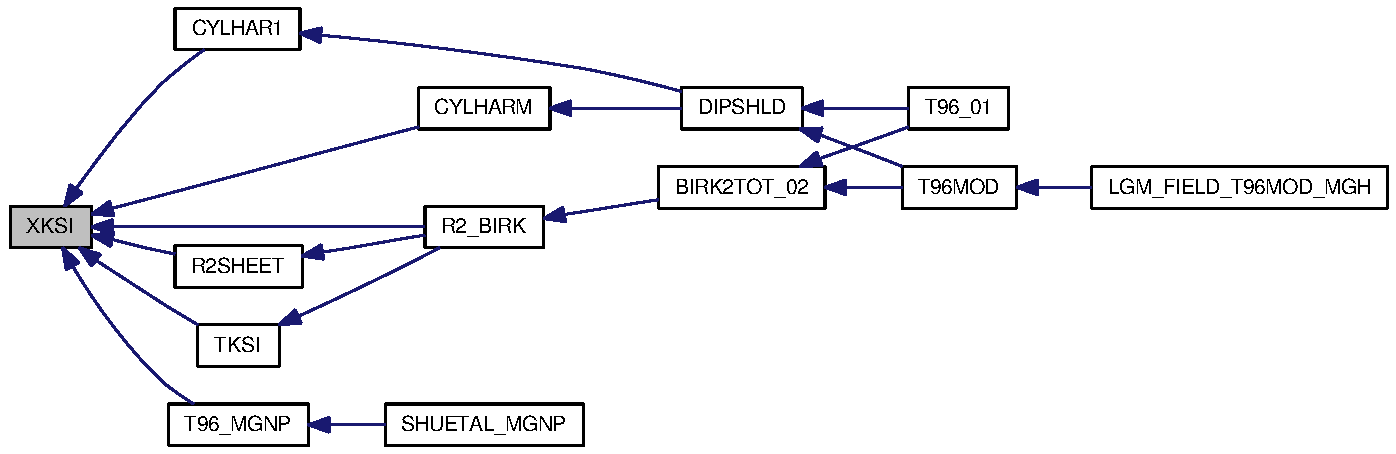
\includegraphics[width=353pt]{_t96mod_8f_34df9615369af608c58c50830a71bc2c_icgraph}
\end{center}
\end{figure}
\hypertarget{_t96mod_8f_de7e8858bac24c4e9ef3bbee7949e235}{
\index{T96mod.f@{T96mod.f}!FEXP@{FEXP}}
\index{FEXP@{FEXP}!T96mod.f@{T96mod.f}}
\subsubsection[{FEXP}]{\setlength{\rightskip}{0pt plus 5cm}function FEXP (S, \/  A)}}
\label{_t96mod_8f_de7e8858bac24c4e9ef3bbee7949e235}




Definition at line 2788 of file T96mod.f.

Here is the caller graph for this function:\nopagebreak
\begin{figure}[H]
\begin{center}
\leavevmode
\includegraphics[width=332pt]{_t96mod_8f_de7e8858bac24c4e9ef3bbee7949e235_icgraph}
\end{center}
\end{figure}
\hypertarget{_t96mod_8f_4652a5d7098ea16cd1f49a0597effa56}{
\index{T96mod.f@{T96mod.f}!FEXP1@{FEXP1}}
\index{FEXP1@{FEXP1}!T96mod.f@{T96mod.f}}
\subsubsection[{FEXP1}]{\setlength{\rightskip}{0pt plus 5cm}function FEXP1 (S, \/  A)}}
\label{_t96mod_8f_4652a5d7098ea16cd1f49a0597effa56}




Definition at line 2797 of file T96mod.f.

Here is the caller graph for this function:\nopagebreak
\begin{figure}[H]
\begin{center}
\leavevmode
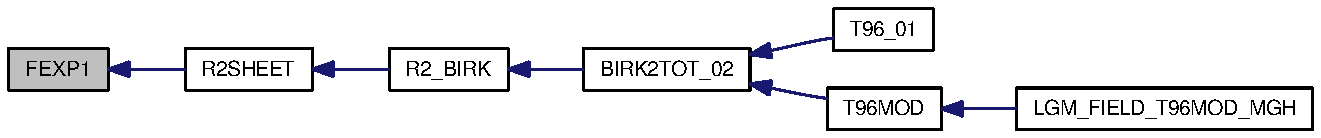
\includegraphics[width=335pt]{_t96mod_8f_4652a5d7098ea16cd1f49a0597effa56_icgraph}
\end{center}
\end{figure}
\hypertarget{_t96mod_8f_2b6a113bedd0458c72d9e0723c3bb7d4}{
\index{T96mod.f@{T96mod.f}!TKSI@{TKSI}}
\index{TKSI@{TKSI}!T96mod.f@{T96mod.f}}
\subsubsection[{TKSI}]{\setlength{\rightskip}{0pt plus 5cm}DOUBLE PRECISION TKSI (XKSI, \/  XKS0, \/  DXKSI)}}
\label{_t96mod_8f_2b6a113bedd0458c72d9e0723c3bb7d4}




Definition at line 2806 of file T96mod.f.

Here is the call graph for this function:\nopagebreak
\begin{figure}[H]
\begin{center}
\leavevmode
\includegraphics[width=80pt]{_t96mod_8f_2b6a113bedd0458c72d9e0723c3bb7d4_cgraph}
\end{center}
\end{figure}


Here is the caller graph for this function:\nopagebreak
\begin{figure}[H]
\begin{center}
\leavevmode
\includegraphics[width=282pt]{_t96mod_8f_2b6a113bedd0458c72d9e0723c3bb7d4_icgraph}
\end{center}
\end{figure}
\hypertarget{_t96mod_8f_39c75fa7da285932d582aadcf8a2442d}{
\index{T96mod.f@{T96mod.f}!T96MOD\_\-DIPOLE@{T96MOD\_\-DIPOLE}}
\index{T96MOD\_\-DIPOLE@{T96MOD\_\-DIPOLE}!T96mod.f@{T96mod.f}}
\subsubsection[{T96MOD\_\-DIPOLE}]{\setlength{\rightskip}{0pt plus 5cm}subroutine T96MOD\_\-DIPOLE (REAL$\ast$8 {\em PS}, \/  REAL$\ast$8 {\em X}, \/  REAL$\ast$8 {\em Y}, \/  REAL$\ast$8 {\em Z}, \/  REAL$\ast$8 {\em BX}, \/  REAL$\ast$8 {\em BY}, \/  REAL$\ast$8 {\em BZ})}}
\label{_t96mod_8f_39c75fa7da285932d582aadcf8a2442d}




Definition at line 2833 of file T96mod.f.

Here is the caller graph for this function:\nopagebreak
\begin{figure}[H]
\begin{center}
\leavevmode
\includegraphics[width=205pt]{_t96mod_8f_39c75fa7da285932d582aadcf8a2442d_icgraph}
\end{center}
\end{figure}
